%%%%%%%%%%%%%%%%%%%%%%%%%%%%%%%%%%%%%%%%%%%%%%%%%%%%%%%%%%%%%%%%%
%%% %
%%% % weiiszablon.tex
%%% % The Faculty of Electrical and Computer Engineering
%%% % Rzeszow University Of Technology diploma thesis Template
%%% % Szablon pracy dyplomowej Wydziału Elektrotechniki 
%%% % i Informatyki PRz
%%% % January, 2024
%%%%%%%%%%%%%%%%%%%%%%%%%%%%%%%%%%%%%%%%%%%%%%%%%%%%%%%%%%%%%%%%%

\documentclass[12pt,twoside]{article}

\usepackage{weiiszablon}
\captionsetup[table]{name=Tabela}
\author{Michał Bazan}

% np. EF-123456, EN-654321, ...
\studentID{EF-163881}

\title{Porównanie wybranych algorytmów nawigacyjnych}
\titleEN{Comparison of selected navigation algorithms}


%%% wybierz rodzaj pracy wpisując jeden z poniższych numerów: ...
% 1 = inżynierska	% BSc
% 2 = magisterska	% MSc
% 3 = doktorska		% PhD
% 4 = praca inżynierska
%%% na miejsce zera w linijce poniżej
\newcommand{\rodzajPracyNo}{2}


%%% promotor
\supervisor{dr inż. Dariusz Rzońca}
%% przykład: dr hab. inż. Józef Nowak, prof. PRz

%%% promotor ze stopniami naukowymi po angielsku
\supervisorEN{Dariusz Rzońca, dr. engineer}

\abstract{Praca koncentruje się na badaniu wybranych algorytmów nawigacyjnych oraz metod optymalizacji nastaw regulatorów PID z wykorzystaniem zbudowanego robota mobilnego, który został skonstruowany zgodnie z procedurami ASPICE. Celem jest ocena dokładności, szybkości wyznaczania trasy oraz ogólnej wydajności tych algorytmów. Analiza wyników pozwoli wyciągnąć wnioski dotyczące skuteczności i efektywności badanych algorytmów nawigacyjnych. Dzięki zastosowaniu standardów ASPICE zapewniona została wysoka jakość procesu budowy robota, co umożliwia rzetelne i wiarygodne badania nad jego funkcjonalnością i algorytmami nawigacyjnymi.}
\abstractEN{Thesis focuses on the study of selected navigation algorithms and methods for optimising PID controller settings using a built mobile robot that has been constructed according to ASPICE procedures. The aim is to evaluate the accuracy, routing speed and overall performance of these algorithms. Analysis of the results will allow conclusions to be drawn regarding the effectiveness and efficiency of the navigation algorithms studied. Through the use of ASPICE standards, the high quality of the robot construction process is ensured, enabling reliable and credible research into its functionality and navigation algorithms.}

\keywords{Algorytmy nawigacyjne, Robot mobilny, Inżynieria, ASPICE, Machine Learning}
\keywordsEN{Navigation algorithms, Mobile robot, Engineering, ASPICE, Machine Learning}


\begin{document}

% strona tytułowa
\maketitle

\blankpage

% spis treści
\tableofcontents

\clearpage
\blankpage


\section*{Wykaz symboli, oznaczeń i skrótów}
\begin{enumerate}[label=\alph*), leftmargin=1.25cm]
	\item PID (eng. Proportional-Integral-Derivative) - skrót od Proporcjonalno-Całkująco-Różniczkującego regulatora, który jest powszechnie stosowany w systemach sterowania,
	\item MCU (eng. Microcontroller Unit) - Jednostka Mikrokontrolera,
	\item SQT (eng. Software Qualification Test) to proces testowania oprogramowania w celu zweryfikowania, czy spełnia ono określone wymagania i standardy jakościowe. SQT ma na celu potwierdzenie, że oprogramowanie działa zgodnie z założeniami i spełnia oczekiwania użytkowników oraz wymagania funkcjonalne i niefunkcjonalne,
	\item GA (eng. Genetic Algorithm) - algorytm genetyczny.
\end{enumerate}

\section{Wstęp}
W dzisiejszych czasach, wraz z dynamicznym rozwojem technologii mobilnych, algorytmy nawigacyjne i uczenia maszynowego \cite{deepLearning} odgrywają kluczową rolę w różnorodnych aplikacjach, począwszy od systemów nawigacji w samochodach po autonomiczne roboty poruszające się w różnych środowiskach. Biorąc pod uwagę aktualność tych zagadnień i rosnące zapotrzebowanie, zdecydowano o przeprowadzeniu badań dotyczących systemów nawigacyjnych.
   
Celem tej pracy jest zbadanie heurystycznych metod \cite{genetics} optymalizacji regulatorów PID oraz wybranych algorytmów pod kątem kryteriów takich jak optymalizacja długości trasy i wydajność obliczeniowa w różnych warunkach terenowych.  

Zakres pracy obejmuje dwie części:
\begin{enumerate}[label=\alph*), leftmargin=1.25cm]
	\item część inżynierska - wykonanie robota mobilnego, implementacja systemu wbudowanego oraz implementacja oprogramowania sterującego robotem poprzez dostępny interfejs sieciowy,
	\item część badawcza - badanie algorytmów uczenia maszynowego do optymalizacji nastaw regulatorów PID oraz porównanie wybranych algorytmów nawigacyjnych. 
\end{enumerate}

Przy realizacji części inżynierskiej zastosowano procedury ASPICE \cite{SPICE}, co  zapewniło wysoką jakość procesu budowy robota oraz implementacji oprogramowania. Takie podejście pozwoliło na przeprowadzenie rzetelnych badań i wyciągnięcie wiarygodnych wniosków.

W następnych rozdziałach pracy przedstawiono szczegółowy opis inżynierskiej części projektu oraz wyniki przeprowadzonych badań. W rozdziale poświęconym inżynierskiej części projektu omówiono budowę robota oraz jego system operacyjny. Komponenty te stanowią podstawę do realizacji badań algorytmicznych. Następnie, w rozdziale dotyczącym badanych algorytmów, zaprezentowano teoretyczne i praktyczne aspekty algorytmu genetycznego, algorytmów nawigacyjnych statycznych oraz dynamicznych. Kolejny rozdział skupia się na opisie przeprowadzonych badań, w których dokonano optymalizacji nastaw regulatora PID oraz przeprowadzono porównanie skuteczności algorytmów nawigacyjnych. Te szczegółowe analizy mają na celu ocenę wydajności poszczególnych rozwiązań oraz identyfikację optymalnych metod nawigacyjnych dla zbudowanego robota.

\section{Inżynierska część projektu}

W tym rozdziale przedstawiono kompleksowy opis prac związanych z implementacją oraz funkcjonowaniem robota. Niniejszy rozdział stanowi szczegółowe omówienie dwóch kluczowych elementów projektu, które skupiały się na budowie fizycznej robota oraz implementacji oprogramowania w języku C++ z uwzględnieniem unit testów.
Dokładna dokumentacja wszystkich komponentów projektu oraz testów znajduje się na repozytorium Github \cite{repo}.

\subsection{Budowa robota}

Pierwszym aspektem, który został przedstawiony, jest proces budowy robota. Opisane zostały tutaj szczegóły dotyczące wyboru komponentów, implementacji elektroniki sterującej oraz budowy konstrukcji mechanicznej. Proces ten obejmuje kilka kluczowych etapów, które mają na celu zapewnienie, że robot będzie w stanie spełniać wszystkie założone funkcje i wymagania. W szczególności skupiono się na doborze odpowiednich czujników, kontrolerów, silników oraz systemu zasilania, które umożliwią robotowi prawidłowe działanie w różnych warunkach.

\subsubsection{Wymagania sprzętowe}

W celu dobrania właściwych elementów do budowy robota sformułowano niżej umieszczone wymagania wysokiego poziomu. Te wymagania określają kluczowe funkcje i cechy, jakie powinny posiadać komponenty sprzętowe robota, aby zapewnić jego pełną funkcjonalność i niezawodność. W tabeli \ref{Tab:HWE1} zestawiono najważniejsze z tych wymagań, które dotyczą obsługi czujników, komunikacji bezprzewodowej, napędu oraz zarządzania zasilaniem.

\begin{table}[ht]
\caption{Wymagania wysokiego poziomu HWE1}
\centering		
	\begin{tabular}{|c|p{0.7\textwidth}|}	
		\hline
		ID\_HWE1 & Opis \\
		\hline
		HWE\_1\_010 & Sprzęt powinien wspierać obsługę czujników odległości. \\
		\hline
		HWE\_1\_020 & Kontroler powinien udostępniać moduł WiFi. \\
		\hline 
		HWE\_1\_030 & Robot powinien być wyposażony w szczotkowe silniki DC z enkoderami.\\
		\hline
		HWE\_1\_040 & Sprzęt powinien wspierać obsługę enkoderów. \\
		\hline
		HWE\_1\_060 & Sprzęt powinien mieć zaimplementowany odpowiedni system dystrybucji zasilania. \\
		\hline

	\end{tabular}	
	
\label{Tab:HWE1}
\end{table}	

\newpage

Na podstawie wymagań wysokiego poziomu ukazanych w tabeli \ref{Tab:HWE1}, sformułowano wymagania niskiego poziomu. Te szczegółowe wymagania określają dokładne specyfikacje techniczne i parametry, które muszą być spełnione przez komponenty, aby zapewnić zgodność z ogólnymi celami projektu. W tabeli \ref{Tab:HWE2} zestawiono kluczowe wymagania dotyczące interfejsów komunikacyjnych, zasilania oraz czujników.


\begin{table}[ht]
\caption{Wymagania niskiego poziomu HWE2}
\centering
\begin{tabular}{|c|p{0.7\textwidth}|}	
    \hline
    ID\_HWE2 & Opis \\
    \hline
    HWE\_2\_010 & Wszystkie interfejsy komunikacyjne powinny wspierać logikę 3V3. \\
    \hline
    HWE\_2\_020 & Mikrokontroler powinien być wyposażony w moduł WiFi. \\
    \hline 
    HWE\_2\_030 & System dystrybucji zasilania powinien zasilić logikę.\\
    \hline
    HWE\_2\_040 & System dystrybucji zasilania powinien zasilić silniki. \\
    \hline
    HWE\_2\_060 & Czujnik odległości powinien mieć zakres pomiarowy wynoszący co najmniej 200 cm. \\
    \hline
    HWE\_2\_070 & Czujniki odległości powinny udostępniać interfejs komunikacyjny kompatybilny z interfejsami mikrokontrolera. \\
    \hline
\end{tabular}
\label{Tab:HWE2}
\end{table}
	

\begin{figure}[ht]%
 \centering%
 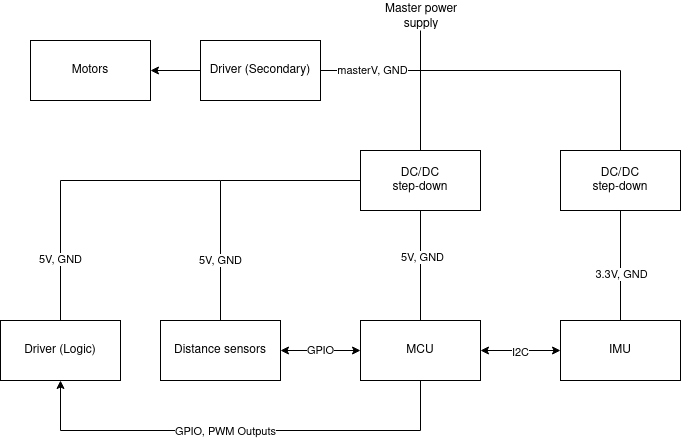
\includegraphics[width=12cm]{figures/engHW/robotblock.png}%
 \caption{Schemat blokowy sprzętu}%
 \label{Fig:schemat}%
\end{figure}

Rysunek \ref{Fig:schemat} ukazuje schemat blokowy utworzony na podstawie wcześniej zdefiniowanych wymagań sprzętowych. Wskazuje, jakie interfejsy i poziomy napięć zasilania zostały wykorzystane pomiędzy poszczególnymi blokami. Sprzęt zdefiniowany w ten sposób oraz zbiór wymagań stawianych przed urządzeniem umożliwił dobór właściwych komponentów.

\newpage

\subsubsection{Schemat elektryczny}
Niniejsza sekcja skupia się na wyjaśnieniu schematu elektrycznego robota. 
Na podstawie umieszczonych w poprzedniej sekcji wymagań dokonano wyboru komponentów, które zostały wykorzystane w projekcie, ale dokładny opis elementów został umieszczony w dokumentacji tej części projektu na repozytorium Github \cite{repo}.\\
\newline
W celu ułatwienia procesu implementacji i zmitygowaniu potencjalnych błędów, schemat elektryczny został podzielony na bloki zgodnie z podziałem ukazanym na rysunku \ref{Fig:schemat}.



\begin{figure}[ht]%
 \centering%
 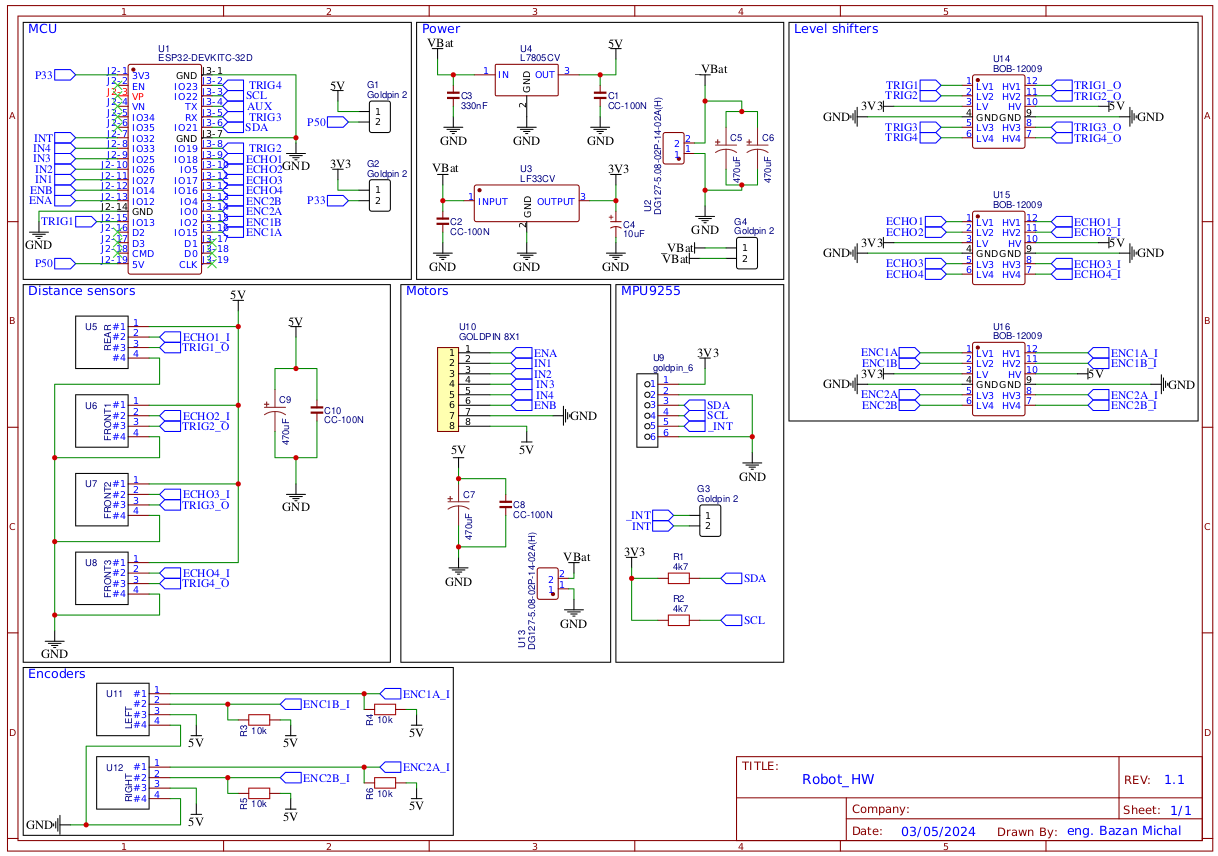
\includegraphics[width=12cm]{figures/engHW/robotschem.png}%
 \caption{Schemat elektryczny}%
 \label{Fig:elektryczny}%
\end{figure}

Rysunek \ref{Fig:elektryczny} ukazuje połączenia pomiędzy blokami schematu:

\begin{enumerate}[label=\alph*), leftmargin=1.25cm]
	\item \textit{MCU} - blok definiuje wejścia i wyjścia sterujące oraz połączenia interfejsów komunikacyjnych,
	\item \textit{Power} - sekcja odpowiedzialna za dystrybucję zasilania,
	\item \textit{Level shifters} - konwertery poziomów logicznych, które zapewniają kompatybilność poziomów sygnałów elektrycznych,
	\item \textit{Distance sensors} - blok definiuje połączenia pomiędzy mikrokontrolerem i czujnikami odległości,
	\item \textit{Motors} - sekcja ukazuje sygnały sterujące silnikami,
	\item \textit{MPU9255} - blok został zaimplementowany, ale nie jest wykorzystywany,
	\item \textit{Encoders} - ta sekcja ukazuje sygnały wyjściowe z enkoderów.
\end{enumerate}

\subsubsection{Testy}
Testowanie tej części projektu polegało głównie na weryfikacji założeń i projektu płytki, dlatego aspekt ten nie został poruszony w tej sekcji. Szczegółowa dokumentacja znajduje się w zdalnym repozytorium \cite{repo}. Testy obejmowały sprawdzenie zgodności z wymaganiami, poprawność połączeń oraz funkcjonalność poszczególnych bloków.

\subsubsection{Konstrukcja mechaniczna}
Konstrukcja mechaniczna robota (rysunek \ref{Fig:robot_const1}) została zaprojektowana jako trzykołowy pojazd, gdzie zastosowano dwa koła sterowalne oraz jedno koło niesterowalne, pełniące funkcję podpory konstrukcji. Komponenty elektroniczne zostały solidnie zamocowane na drewnianej płycie montażowej. Położenie każdego elementu zostało starannie zaplanowane w celu maksymalnego wykorzystania dostępnej przestrzeni. Kluczowym aspektem było minimalizowanie odległości między poszczególnymi blokami, co pozwoliło uniknąć problemów z połączeniami i zapewniło efektywną integrację bloków funkcjonalnych robota. Projekt konstrukcji uwzględniał również ergonomiczne rozmieszczenie elementów w celu ułatwienia dostępu do poszczególnych części w przypadku konserwacji i napraw. Dzięki szczegółowemu planowaniu, robot nie tylko spełniał wymagania funkcjonalne, ale również charakteryzował się kompaktowym i przejrzystym układem komponentów, co zwiększało jego niezawodność i łatwość obsługi. Rysunek \ref{Fig:robot_const2} ukazuje rozmieszczenie bloków funkcjonalnych robota:
\begin{enumerate}[label=\alph*), leftmargin=1.25cm]
	\item czujnik odległości tył,
	\item płytka z mikrokontrolerem odpowiedzialna za komunikację i sterowanie blokami,
	\item silniki prądu stałego z enkoderami,
	\item dwukanałowy sterownik silników prądu stałego,
	\item akumulatory zasilające elektronikę i silniki,
	\item czujniki odległości przód.
\end{enumerate}

\begin{figure}[ht]%
 \centering%
 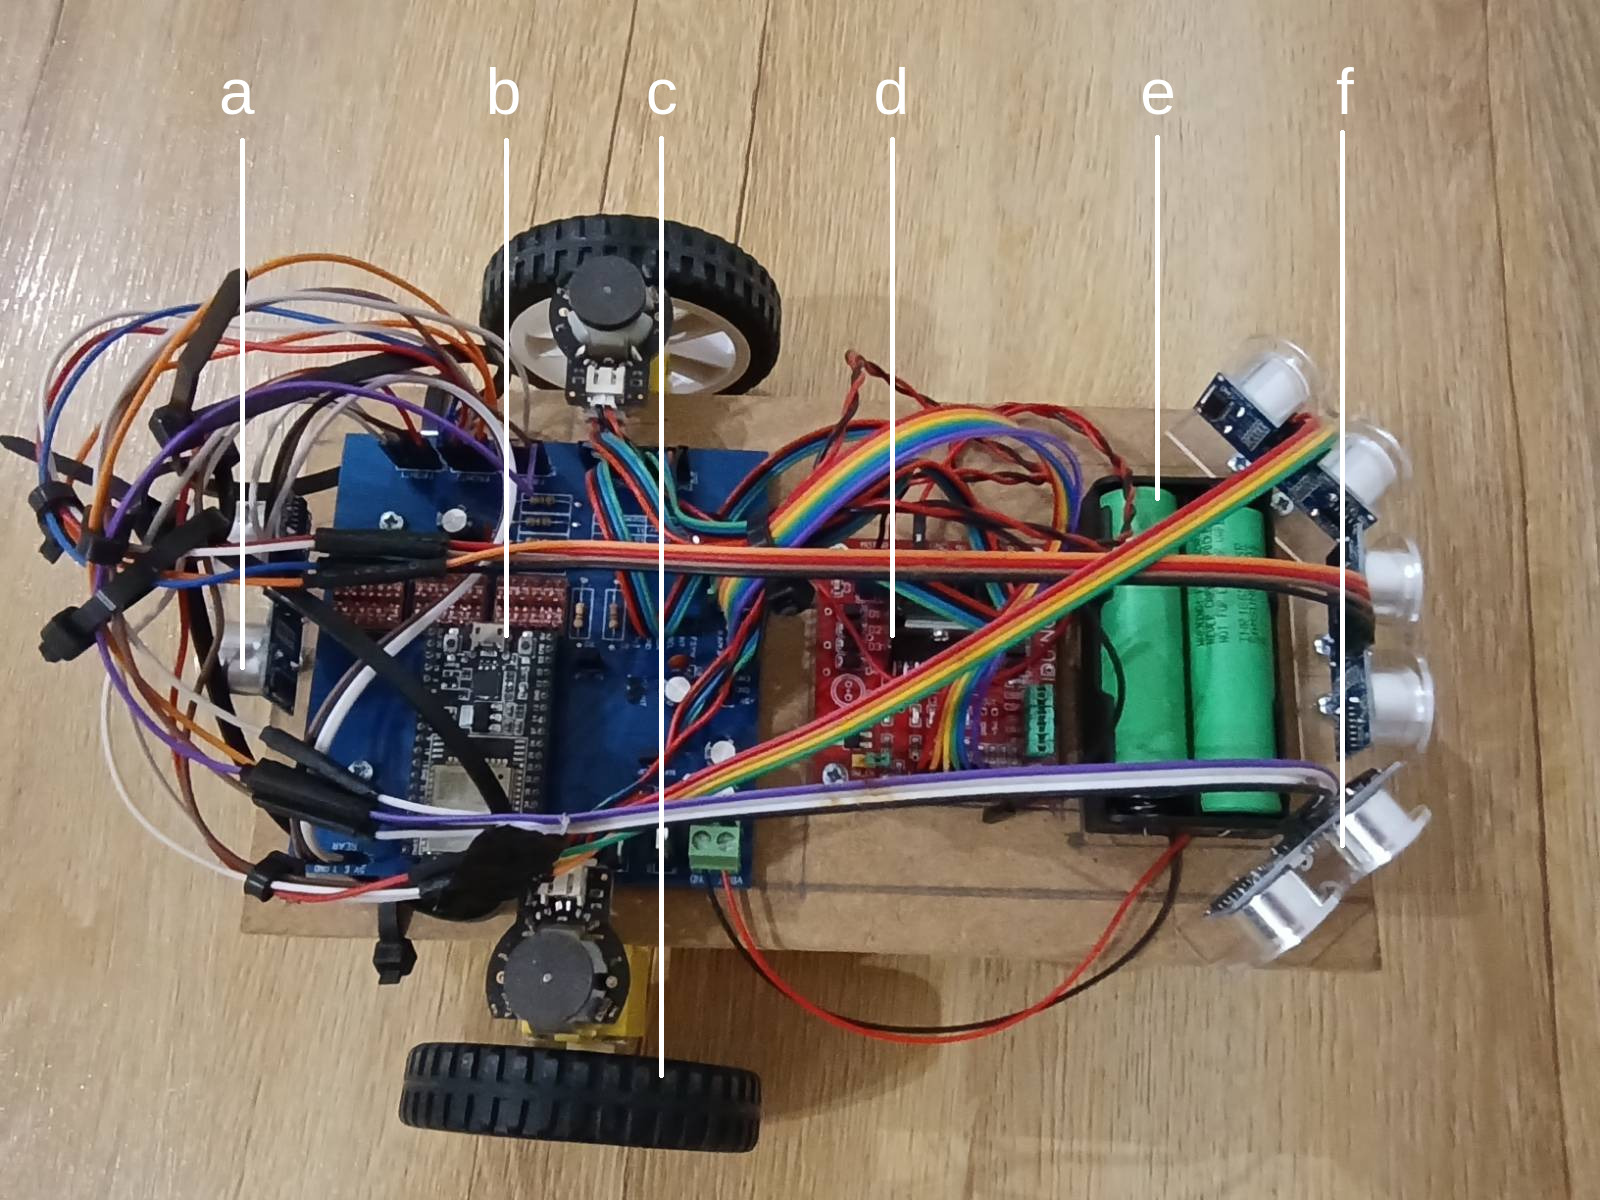
\includegraphics[width=9cm]{figures/robot/robot_up.jpg}%
 \caption{Rozmieszczenie bloków}%
 \label{Fig:robot_const2}%
\end{figure}



\begin{figure}[ht]%
 \centering%
 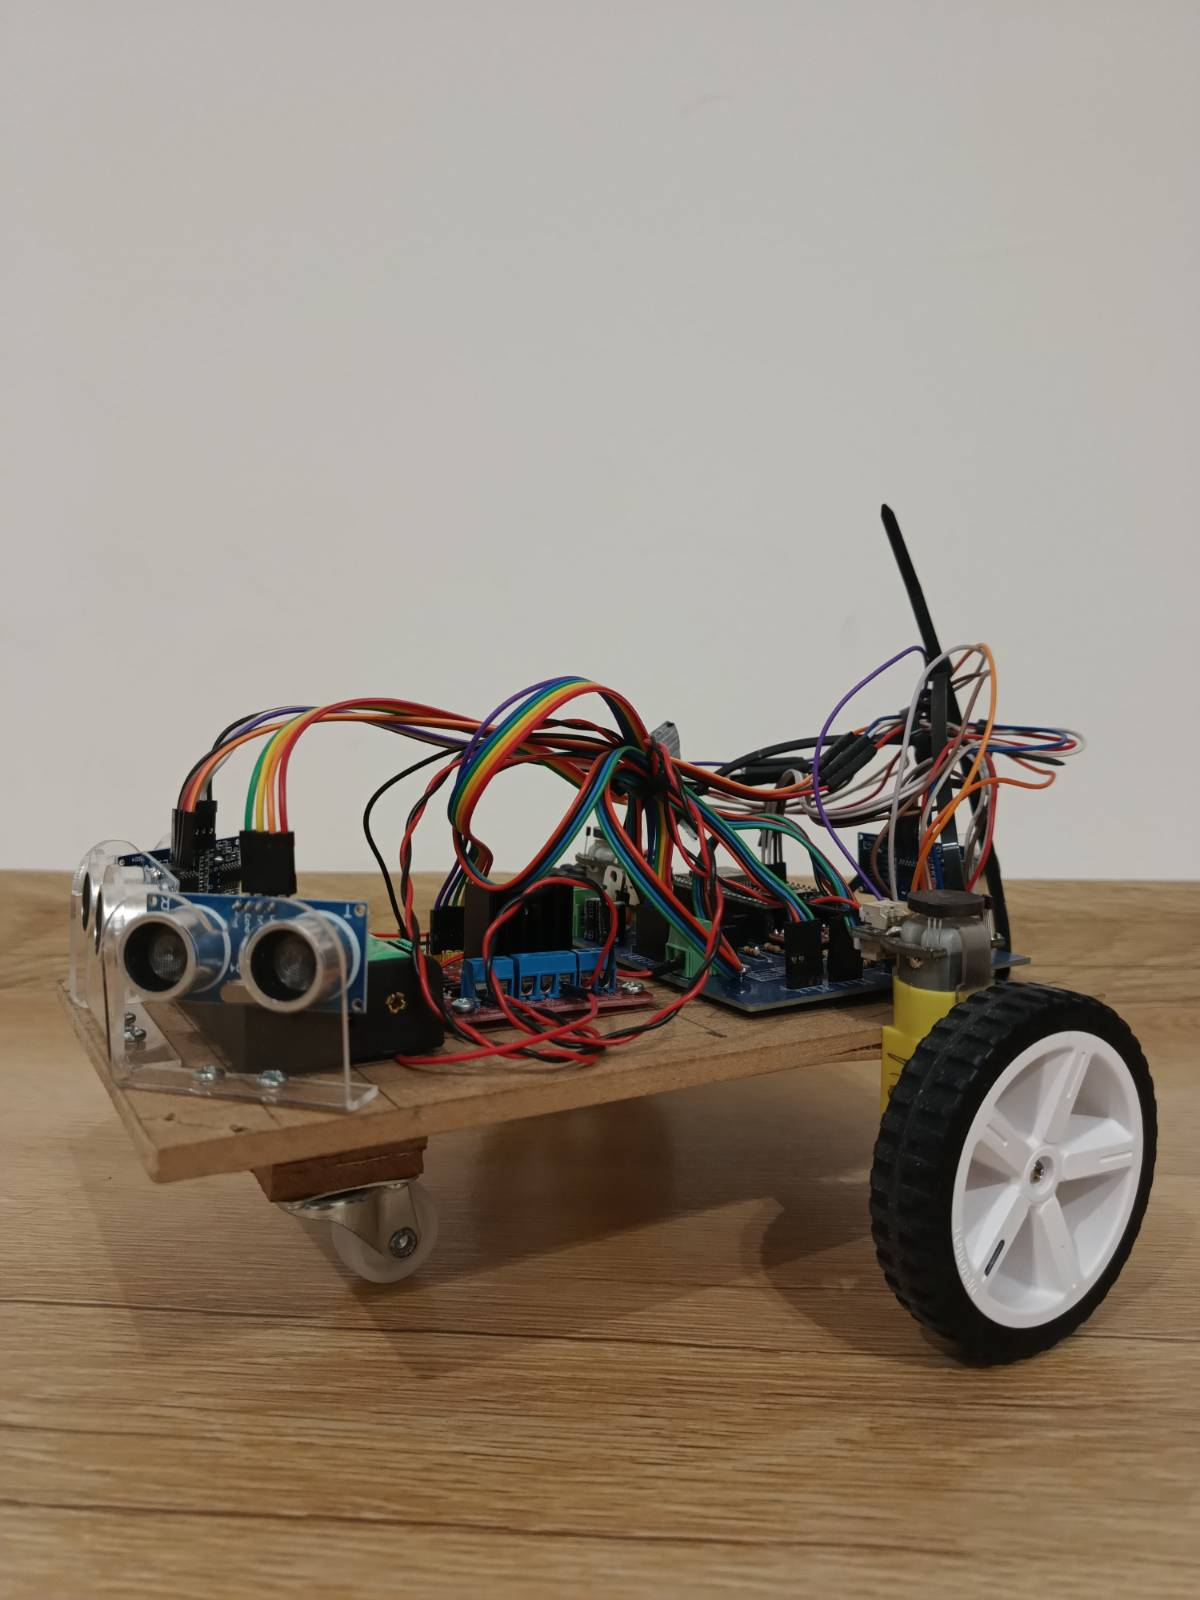
\includegraphics[width=9cm]{figures/robot/robot2.jpg}%
 \caption{Wykonany robot mobilny}%
 \label{Fig:robot_const1}%
\end{figure}

\clearpage

\subsection{System operacyjny robota}

Niniejsza sekcja skupia się na implementacji oprogramowania w języku C++\cite{cpp}, obejmującej zarówno projektowanie, jak i implementację funkcjonalności. System operacyjny robota zarządza wszystkimi aspektami operacyjnymi robota, od odczytu danych z czujników, poprzez przetwarzanie i analizę tych danych, aż po sterowanie silnikami i komunikację  przez interfejs sieciowy.

\subsubsection{Wymagania dotyczące oprogramowania}

Na podstawie wcześniej omówionych wymagań sprzętowych oraz celów tego projektu, sformułowano następujące wymagania wysokiego poziomu (tabela \ref{Tab:SWE2}). Wymagania te definiują kluczowe funkcjonalności, jakie powinno posiadać oprogramowanie, aby zapewnić niezawodność działania robota.

\begin{table}[ht]
\caption{Wymagania wysokiego poziomu SWE2}
\centering		
	\begin{tabular}{|c|p{0.7\textwidth}|}	
		\hline
		ID\_SWE2 & Opis \\
		\hline
		SWE\_2\_010 & Oprogramowanie powinno odczytywać sensory periodycznie. \\
		\hline
		SWE\_2\_020 & Interfejs WiFi powinien być wykorzystany do komunikacji z oprogramowaniem sterującym. \\
		\hline 
		SWE\_2\_030 & Oprogramowanie powinno udostępniać interfejs do sterowania silnikami.\\
		\hline
		SWE\_2\_040 & Komunikacja powinna wykorzystywać prosty protokół komunikacyjny do wymiany danych pomiędzy robotem a oprogramowaniem sterującym. \\
		\hline
		SWE\_2\_050 & Oprogramowanie powinno implementować algorytm wyznaczający odometrię. \\
		\hline

	\end{tabular}	
	
\label{Tab:SWE2}
\end{table}	

W celu wyłonienia konkretnych bloków, z jakich powinno składać się oprogramowanie, zdefiniowano następujące wymagania niskiego poziomu (tabela \ref{Tab:SWE3}). Te szczegółowe wymagania określają specyficzne zadania i interfejsy, które muszą być zaimplementowane, aby spełnić założenia projektowe.

\begin{table}[ht]
\caption{Wymagania niskiego poziomu SWE3}
\centering		
	\begin{tabular}{|c|p{0.7\textwidth}|}	
		\hline
		ID\_SWE3 & Opis \\
		\hline
		SWE\_3\_010 & Oprogramowanie powinno odczytywać sensory co 50ms. \\
		\hline
		SWE\_3\_020 & Oprogramowanie powinno udostępniać interfejs do wymiany danych. \\
		\hline 
		SWE\_3\_030 & Oprogramowanie powinno udostępniać dane z sensorów na żądanie.\\
		\hline
		SWE\_3\_040 & Komunikacja powinna opierać się o wykorzystanie protokołu MQTT. \\
		\hline
		SWE\_3\_050 & Oprogramowanie powinno udostępnić interfejs do sterowania silnikami. \\
		\hline
		SWE\_3\_060 & Implementacja powinna wykorzystywać prostą odometrię. \\
				\hline
	\end{tabular}	
	
\label{Tab:SWE3}
\end{table}	

\newpage

\begin{figure}[ht]%
 \centering%
 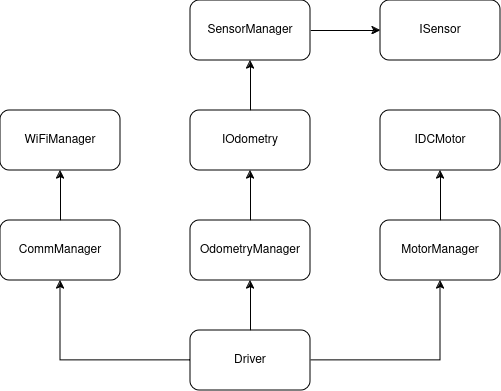
\includegraphics[width=12cm]{figures/engSW/block.png}%
 \caption{Architektura oprogramowania}%
 \label{Fig:architektura}%
\end{figure}

Na rysunku \ref{Fig:architektura} przedstawiono architekturę systemu operacyjnego robota, która została zaprojektowana w oparciu o wcześniej zdefiniowane wymagania niskiego poziomu (tabela \ref{Tab:SWE3}). Architektura ta składa się z kilku kluczowych modułów:

\begin{enumerate}[label=\alph*), leftmargin=1.25cm]
	\item \textit{CommManager} - odpowiada za połączenie sieciowe i komunikację za pośrednictwem protokołu MQTT,
	\item \textit{SensorManager} - posiada uchwyt do wszystkich dostępnych sensorów, które obsługuje periodycznie,
	\item \textit{OdometryManager} - posiada uchwyt do obiektu typu \textit{SensorManager} i realizuje odometrię na podstawie odczytów z czujników,
	\item \textit{MotorManager} - steruje silnikami zależnie od nadchodzących komunikatów,
	\item \textit{Driver} - odpowiada za poprawną inicjalizację systemu, wywoływanie funkcji callbackowych z bloku odpowiedzialnego za komunikację oraz ustawienie prędkości obrotowej silników zależnie od uchybu regulacji.  
\end{enumerate}

\subsubsection{Implementacja}
Implementacja systemu operacyjnego robota składa się z 12 klas, z których każda pełni określoną rolę w funkcjonowaniu robota. Klasy te zarządzają różnymi aspektami operacyjnymi, od odczytu danych z czujników po sterowanie silnikami. Ważnym elementem implementacji jest również prosty szablon regulatora PID oraz stos oparty na \textit{std::array}\cite{stdarray}.

\begin{lstlisting}[language=C++, caption={Klasa CommManager}, label={lst:CommManager}]
template<class StringType, std::size_t topic_num>
class CommManager{
public:
    using messageType = std::tuple<StringType, StringType>;
    using onMsg_cb = std::function<void(char*, byte*, unsigned int)>;

    static messageType createMessage(const StringType& topic, const StringType& payload) noexcept;

    CommManager(
        WiFiManager<StringType>&& w, 
        const StringType& uname, 
        const StringType& broker, 
        const StringType& password, 
        WiFiClient& c, 
        std::array<StringType, topic_num>&& topics,
        const onMsg_cb& cback,
        const StringType& ID = "Robot"
        ) noexcept;

    MQTTStatus poolCommManager() noexcept;
    
    bool sendMessage(messageType&& message) noexcept;

private:
    NetworkStatus poolNetwork() noexcept;
    SemaphoreHandle_t MQTTQueueMutex;

    enum : uint8_t{
        ConnectingNetwork = 0,
        ConnectingBroker,
        Timeout,
        CheckingStatus
    };
    uint8_t m_internalState;
    WiFiManager<StringType> m_wifiMgr;
    custom::stack<messageType, stack_depth> m_messageStack;
    StringType m_broker;
    StringType m_password;
    StringType m_uname;
    StringType m_ID;
    const std::array<StringType, topic_num> m_topics;
    PubSubClient m_mqttClient;
    onMsg_cb m_message_cb;
};
\end{lstlisting}

Klasa \textit{CommManager} (listing \ref{lst:CommManager}) zarządza komunikacją między robotem a oprogramowaniem sterującym poprzez protokół MQTT i połączenie WiFi. Oferuje funkcje odczytu danych z czujników, wysyłania komunikatów i reakcji na przychodzące komunikaty. Metoda \textit{createMessage} tworzy nową wiadomość MQTT na podstawie tematu i treści. W konstruktorze inicjalizowane są połączenie WiFi, parametry MQTT i lista subskrybowanych tematów. \textit{poolCommManager} zarządza połączeniem z WiFi i brokerem MQTT, podejmując odpowiednie działania w zależności od stanu połączenia. \textit{sendMessage} dodaje wiadomość do kolejki komunikatów. Klasa zapewnia niezawodne połączenie i efektywną komunikację, co jest kluczowe dla funkcjonowania robota w różnych scenariuszach działania.

\begin{lstlisting}[language=C++, caption={Klasa SensorManager}, label={lst:SensorManager}]
enum class SensorMapping : uint8_t{ 
    LEFT_Encoder,
    RIGHT_Encoder,
    DST_Front_1,
    DST_Front_2,
    DST_Front_3,
    DST_Rear
};

constexpr uint8_t translate(SensorMapping s){
    return static_cast<uint8_t>(s);
}

class SensorManager{
public:
    void init();
    SensorManager(std::array<sensorPointer, numSensors>&& s);
    void poolSensors();
    ISensor& getSensor(SensorMapping s);

private:
    std::array<sensorPointer, numSensors> sensors;
};
\end{lstlisting}

Klasa \textit{SensorManager} (listing \ref{lst:SensorManager}) zarządza sensorami robota przechowując ich wskaźniki i udostępniając interfejs odczytu danych. Typ \textit{SensorMapping} reprezentuje indeksy sensorów, ułatwiając dostęp do nich. Metoda \textit{translate} przekształca enumerator na liczby całkowite, co umożliwia łatwiejszy dostęp do konkretnego urządzenia. Konstruktor inicjuje obiekt tablicą uchwytów reprezentujących urządzenia, a \textit{init} inicjuje sensory. Metoda \textit{poolSensors} odpytuje sensory, a \textit{getSensor} zwraca referencję do konkretnego sensora.

\newpage

\begin{lstlisting}[language=C++, caption={Klasa OdometryManager}, label={lst:OdometryManager}]
enum ActiveOdometry : std::size_t {
    SimpleOdo = 0,
    AdvancedOdo = 1
};

constexpr std::size_t availableAlgorithms = 2;

class OdometryManager{
public:
    OdometryManager(
        std::array<IOdometry*, availableAlgorithms>&& odo,
        SensorManager& s
    ) noexcept;

    void updatePosition() noexcept;
    void setActiveOdometry(ActiveOdometry o) noexcept;
    std::size_t getActiveOdometry() const noexcept;
    const position getPosition() const noexcept;
    void resetActiveOdometry() noexcept;
private:
    std::array<IOdometry*, availableAlgorithms> m_odometryAgents;
    SensorManager& m_sensorMgr;
    std::size_t m_active;
};
\end{lstlisting}

Klasa \textit{OdometryManager} (listing \ref{lst:OdometryManager}) zarządza różnymi algorytmami odometrii robota i aktualizuje jego pozycję na podstawie danych z sensorów. Enumerator \textit{ActiveOdometry} definiuje dostępne algorytmy odometrii, lecz w tej implementacji dostępna jest tylko prosta odometria. Konstruktor przyjmuje tablicę wskaźników do obiektów \textit{IOdometry} reprezentujących różne algorytmy odometrii oraz referencję do obiektu \textit{SensorManager}. Metoda \textit{updatePosition} aktualizuje pozycję robota na podstawie danych z sensorów i aktywnego algorytmu odometrii. \textit{setActiveOdometry} ustawia aktywny algorytm odometrii, \textit{getActiveOdometry} zwraca jego indeks, a \textit{getPosition} zwraca aktualną pozycję. Metoda \textit{resetActiveOdometry} resetuje aktywny algorytm i ustawia zerowe współrzędne. Klasa zapewnia elastyczne zarządzanie algorytmem odometrii i precyzyjne poruszanie się robota.


\begin{lstlisting}[language=C++, caption={Klasa MotorManager}, label={lst:MotorManager}]
class MotorManager{
public:
    enum class settingType{
        setAngularTarget,
        updatePwm
    };

    using motor_array = std::array<IDCMotor*, motor_num>;
    using speed_array = std::array<int32_t, motor_num>; 
    using angular_array = std::array<float, motor_num>;

    void init() noexcept;
    void setSpeed(const speed_array& speeds, settingType t = settingType::updatePwm) noexcept;
    MotorManager(motor_array&& m, float i = inertia_coef) noexcept;
    void InertiaCoef(float i) noexcept;
    float InertiaCoef() const noexcept;
    void poolMotors() noexcept;
    const speed_array* CurrentSpeed() const noexcept;
    const speed_array* DesiredSpeed() const noexcept;
    const angular_array* TargetAngular() const noexcept;

private:
    float m_inertiaCoef;
    motor_array motors;
    speed_array target_percent_speed;
    speed_array current_percent_speed;
    angular_array target_angular_speed;
};
\end{lstlisting}

Klasa \textit{MotorManager} (listing \ref{lst:MotorManager}) zarządza silnikami prądu stałego robota, kontrolując ich prędkość obrotową i kierunek. \textit{settingType} definiuje różne typy ustawień silników, a \textit{motor\_array}, \textit{speed\_array}, i \textit{angular\_array} to odpowiednio tablice wskaźników do silników, prędkości silników i prędkości kątowych. Metoda \textit{init} inicjuje silniki, \textit{setSpeed} ustawia prędkość zależnie od typu ustawienia, a konstruktor inicjuje obiekt, przyjmując tablicę wskaźników do silników i opcjonalny współczynnik inercji. \textit{poolMotors} aktualizuje stany silników, a \textit{CurrentSpeed}, \textit{DesiredSpeed}, i \textit{TargetAngular} zwracają odpowiednio aktualną prędkość, docelową prędkość i prędkości kątowe silników. Klasa zapewnia elastyczne zarządzanie silnikami i kontrolę nad ich prędkościami, kluczową dla ruchu i sterowania robotem.

\begin{lstlisting}[language=C++, caption={Klasa Kernel}, label={lst:Kernel}]
class Kernel{
public:
    static void init();
    static void main();
    
    /* motion management */
    static Motor::DCMotor motorLeft;
    static Motor::DCMotor motorRight;
    static Motor::MotorManager motorManager;
    static uint32_t mapper(uint32_t);
    static constants::motors::types::motor_pid pidLeft;
    static constants::motors::types::motor_pid pidRight;

    /* communications management */
    static constants::comm::types::job_stack_t jobStack;
    static Comm::MQTT::CommManager<String, constants::comm::subscribedTopics> commMgr;
    static void MQTTcallback(char*, byte*, unsigned int);

    /* sensor management */
    static Sensor::DistanceSensor rear;
    static Sensor::DistanceSensor front_left;
    static Sensor::DistanceSensor front;
    static Sensor::DistanceSensor front_right;
    static Sensor::Encoder encoderLeft;
    static Sensor::Encoder encoderRight;

    static Sensor::SensorManager sensorMgr;

    static Sensor::simpleOdometry odoAgent;
    static Sensor::OdometryManager odoMgr;
};    
\end{lstlisting}

Klasa \textit{Kernel} (listing \ref{lst:Kernel}) pełni kluczową rolę jako centralny moduł zarządzający systemem. Odpowiada za inicjalizację systemu oraz koordynację jego głównych funkcji. Metoda \textit{init} przygotowuje system do działania, a \textit{main} zarządza jego główną logiką. Kluczowe funkcje obejmują zarządzanie ruchem (silniki, regulator PID), komunikacją (MQTT), sensorami (odległości, enkodery) oraz odometrią. \textit{Kernel} integruje te komponenty, zapewniając ich współpracę i efektywny podział czasu procesora.

\subsubsection{Obsługiwane polecenia}

Sekcja przedstawia interfejs sieciowej komunikacji z robotem poprzez protokół MQTT. Tabela \ref{Tab:RobotSub} zawiera tematy subskrybowane przez robota wraz z opisem ich przeznaczenia oraz przykładowymi danymi. Tabela ta obejmuje kanały do debugowania, przesyłania komend oraz ustawiania prędkości silników. Natomiast w tabeli \ref{Tab:RobotPub} przedstawione zostały tematy publikowane przez robota wraz z opisem i typowymi danymi przesyłanymi przez te kanały takie jak odpowiedzi na komendy i wiadomości służące do debugowania. W tabeli \ref{Tab:RobotCMD} znajdują się dostępne komendy, ich opisy oraz oczekiwane odpowiedzi. Komendy obejmują pobieranie odczytów z czujników, resetowanie pozycji, pobieranie danych odometrycznych oraz zatrzymywanie silników.

\begin{table}[ht]
\caption{Tematy subskrybowane przez robota}
\centering		
	\begin{tabular}{|p{0.2\textwidth}|p{0.4\textwidth}|p{0.3\textwidth}|}	
		\hline
		Robot subskrybuje & Opis & Dane \\
		\hline
		robot/echo/in & Temat wykorzystywany do debugu, system odpowiada ciągiem tekstowym na temacie robot/echo/out. & Dowolny ciąg tekstowy zgodny z ASCII. \\
		\hline
		robot/cmd/in & Temat do przesyłania zdefiniowanych komend (tab. \ref{Tab:RobotCMD} ). & Komenda jako ciąg tekstowy zgodny z ASCII. \\
		\hline
		robot/set/motors & Temat do przesyłania żądanych prędkości silników. & Dane w formacie JSON: \{ „left” : x, „right” : y \}, gdzie x oraz y to prędkości wyrażone w procentach. \\
		\hline
	\end{tabular}	
	
\label{Tab:RobotSub}
\end{table}	

\begin{table}[ht]
\caption{Tematy publikowane przez robota}
\centering		
	\begin{tabular}{|p{0.2\textwidth}|p{0.4\textwidth}|p{0.3\textwidth}|}	
		\hline
		Robot subskrybuje & Opis & Dane \\
		\hline
		robot/echo/out & Temat, na który system przesyła wiadomości dotyczące debugu. & Dowolny ciąg tekstowy zgodny z ASCII. \\
		\hline
		robot/cmd/response & Odpowiedź na przesłaną komendę. & Dane w formacie JSON (odczyty z sensorów, odometria), brak odpowiedzi lub ciąg tekstowy 'cmd not supported' w przypadku przesłania błędnej komendy. \\
		\hline
	\end{tabular}	
	
\label{Tab:RobotPub}
\end{table}	

\begin{table}[ht]
\caption{Dostępne komendy}
\centering		
	\begin{tabular}{|p{0.2\textwidth}|p{0.4\textwidth}|p{0.3\textwidth}|}	
		\hline
		Komenda & Opis & Odpowiedź \\
		\hline
		get\_sensors & Pobierz odczyty z czujników. & Dane z czujników w formacie JSON. \\
		\hline
		reset\_odo & Zeruj pozycję. & Brak odpowiedzi. \\
		\hline
		get\_odo & Pobierz wyznaczone dane odometryczne. & Dane w formacie JSON. \\
		\hline
		get\_all & Pobierz dane z sensorów i pozycję robota. & Dane w formacie JSON. \\
		\hline
		halt & Zatrzymaj silniki. & Brak odpowiedzi. \\
		\hline
	\end{tabular}	
	
\label{Tab:RobotCMD}
\end{table}	

\newpage
\subsubsection{Testy oprogramowania}
Niniejsza sekcja skupia się na opisie przeprowadzonych testów weryfikujących zgodność oprogramowania z wymaganiami określonymi w specyfikacji SWE3.

\begin{table}[ht]
\caption{Test SQT\_01}
\centering		
	\begin{tabular}{|p{0.2\textwidth}|p{0.4\textwidth}|p{0.3\textwidth}|}	
		\hline
		Treść wymagania & Weryfikacja & Wynik testu \\
		\hline
		Oprogramowanie powinno odczytywać sensory co 50ms. & Zadanie odczytywania sensorów jest zaplanowane w systemie freeRTOS co 50ms. & Wynik pozytywny \\
		\hline
	\end{tabular}	
	
\label{Tab:TEST1}
\end{table}	

\begin{table}[ht]
\caption{Test SQT\_02}
\centering		
	\begin{tabular}{|p{0.3\textwidth}|p{0.3\textwidth}|p{0.3\textwidth}|}	
		\hline
		Weryfikacja & Oczekiwane & Obserwacja \\
		\hline
		Podłączenie płytki do zasilania &
		Płytka powinna być poprawnie zasilona &
		Płytka została poprawnie zasilona \\
		\hline
		Wgranie najnowszej wersji oprogramowania na płytkę &
		Najnowsze oprogramowanie powinno zostać wgranę na płytkę &
		Najnowsze oprogramowanie zostało wgrane na płytkę \\
		\hline
		Oczekiwanie na wiadomość 'robot initialized' na temacie robot/echo/out. &
		Wiadomość powinna zostać odebrana. &
		Wiadomość została odebrana. \\
		\hline
		Przesłanie wiadomości na temacie robot/set/motors, aby ustawić prędkość silników bliską 40\% prędkości maksymalnej. 			&
		Silniki powinny kręcić się z prędkością bliską 40\% prędkości maksymalnej. &
		Silniki kręcą się z prędkością bliską 40\% prędkości maksymalnej. \\
		\hline
		Przesłanie komendy 'halt' na temacie robot/cmd/in. &
		Silniki powinny się zatrzymać. &
		Silniki zatrzymały się. \\
		\hline
		Przesłanie komendy 'get\_all' w celu uzyskania wszystkich danych. &
		Uzyskano dane z sensorów i pozycję robota. &
		Uzyskano dane z sensorów i pozycję robota. \\
		\hline
		Przesłanie komendy 'reset\_odo' w celu resetowania odometrii. &
		Wiadomość powinna zostać wysłana. &
		Wiadomość została wysłana. \\
		\hline
		Przesłanie komendy 'get\_odo' w celu uzyskania pozycji robota. &
		Uzyskano pozycję, która wskazuje na zero. &
		Uzyskano pozycję, która wskazuje na zero. \\
		\hline
	\end{tabular}	
	
\label{Tab:TEST1}
\end{table}	
\newpage

Test \textit{SQT\_01} miał na celu potwierdzenie, czy oprogramowanie regularnie odczytuje dane z czujników odległości co 50 ms, zgodnie z wymaganiami. Mimo że w projekcie nie wykorzystano IMU, to test został dostosowany do odczytu danych z czujników odległości, a zadanie zostało zaplanowane jako praca \textit{freeRTOS} \cite{freeRTOS} z interwałem 50 ms.

Testy oznaczone jako \textit{SQT\_02} skupiły się na weryfikacji podstawowych funkcji oprogramowania, w tym dostarczania zasilania i programowania sprzętu, wymiany danych, kontroli silników itp. Każde z tych wymagań zostało poddane testowi, a wynikiem było potwierdzenie, że oprogramowanie spełnia te kryteria.

W obu przypadkach testy zakończyły się sukcesem, co potwierdza zgodność oprogramowania z wymaganiami określonymi w specyfikacji SWE3. Oprócz przeprowadzenia testów kwalifikacyjnych oprogramowanie zostało pokryte testami jednostkowymi.

\clearpage

\section{Wprowadzenie do omawianych algorytmów}

\subsection{Algorytm PID}
Algorytm PID \cite{PID} jest podstawowym narzędziem używanym w systemach sterowania. Celem tego regulatora jest minimalizacja różnicy między wartością zadaną a rzeczywistą wartością procesu poprzez odpowiednie dostosowanie sygnału sterującego. Regulator PID składa się z trzech komponentów (wzór \ref{Eq:rownaniePID}):



\begin{enumerate}[label=\alph*), leftmargin=1.25cm]
	\item składnik proporcjonalny (wzór \ref{Eq:rownanieP}) - generuje sygnał sterujący proporcjonalny do bieżącego błędu. Wyższa wartość współczynnika wzmocnienia prowadzi do szybszej reakcji systemu, ale może powodować oscylacje lub niestabilność,
	
	\item składnik całkujący (wzór \ref{Eq:rownanieI}) - eliminuje stałe odchylenie przez sumowanie błędów w czasie. Powoduje to wzrost sygnału sterującego, dopóki błąd nie zostanie zredukowany do zera. Współczynnik nie powinien być zbyt duży, ponieważ może powodować przeregulowania i oscylacje,
	
	\item składnik różniczkujący (wzór \ref{Eq:rownanieD}) - reaguje na szybkość zmiany odpowiednio korygując sygnał sterujący. Pomaga w tłumieniu oscylacji i poprawia stabilność systemu. Zbyt duża wartość wzmocnienia może jednak sprawić, że regulator będzie zbyt agresywnie zmieniał wartość sterującą.
\end{enumerate}

\begin{equation}
P = K_p \cdot e(t)
\label{Eq:rownanieP}
\end{equation}

\begin{equation}
I = K_i \cdot \int_0^t \cdot e(\tau)d\tau
\label{Eq:rownanieI}
\end{equation}

\begin{equation}
D = K_d \cdot \frac{de(t)}{dt}
\label{Eq:rownanieD}
\end{equation}


\begin{equation}
PID = K_p \cdot e(t) + K_i \cdot \int_0^t \cdot e(\tau)d\tau + K_d \cdot \frac{de(t)}{dt}
\label{Eq:rownaniePID}
\end{equation}

gdzie: $K_p$ -- wzmocnienie członu proporcjonalnego, $K_i$ -- wzmocnienie członu całkującego, $K_d$ -- wzmocnienie członu różniczkującego, $e(t)$ -- błąd regulacji \\

W regulatorze analogowym PID wszystkie operacje matematyczne są wykonywane w sposób ciągły przy użyciu komponentów elektronicznych takich jak oporniki, kondensatory i wzmacniacze operacyjne. Ze względu na wykorzystane technologie, w prezentowanym rozwiązaniu zastosowana została dyskretna wersja algorytmu, która w porównaniu do regulatora ciągłego, ograniczona jest niższą dokładnością całkowania i różniczkowania.

\lstset{language=C++}

\begin{lstlisting}[caption={Kod implementacji cyfrowego algorytmu PID}, label={lst:pid_algorithm}]
template <typename ValueType, typename outType, outType MaxOut, outType MinOut, int32_t maxErrorSum, int32_t minErrorSum, uint32_t samplingMs = 20>
class pid{
public:
    /*
        Kp - proportional Gain
        Ti - integrator constant
        Td - derivative constant
        Ts - sampling time in ms
    */
    constexpr pid(float Kp, float Ti, float Td) noexcept:
        m_Kp{ Kp }, m_Ki{ (Kp / Ti) * (samplingMs * 0.001f) }, m_Kd{ (Kp * Td)/(samplingMs * 0.001f + 0.1f*Td) },
        m_errorSum{ 0 }, m_previousError{ 0 } {}
    
    void reinit(float Kp, float Ti, float Td){
        m_Kp = Kp;
        m_Ki = (Kp / Ti) * (samplingMs * 0.001f);
        m_Kd = (Kp * Td)/((samplingMs * 0.001f) + 0.1f*Td);
        m_errorSum = m_previousError = 0;
    }

    outType getOutput(ValueType actual, ValueType desired){
        auto error = desired - actual;
        float P = m_Kp * error;
        
        m_errorSum += static_cast<int32_t>(error);

        if(m_errorSum > maxErrorSum){
            m_errorSum = maxErrorSum;
        }
        else if(m_errorSum < minErrorSum){
            m_errorSum = minErrorSum; 
        }

        float I = m_Ki * m_errorSum;
        float D = m_Kd * (error - m_previousError);

        auto output = static_cast<outType>(P + I + D);

        if(output > MaxOut){
            return MaxOut;
        }
        else if(output < MinOut){
            return MinOut;
        }
        else{
            return output;
        }
    }

private:
    float m_Kp;
    float m_Ki;
    float m_Kd;
    ValueType m_errorSum;
    ValueType m_previousError;
};
\end{lstlisting}

Kod ukazany na listingu \ref{lst:pid_algorithm} definiuje szablon klasy \textit{pid}, który reprezentuje cyfrowy algorytm PID. Kluczowymi elementami tego algorytmu są trzy główne składowe: proporcjonalny, całkujący i różniczkujący.

Algorytm ten jest parametryzowany przez wartości takie jak wzmocnienia (\textit{Kp}, \textit{Ki}, \textit{Kd}) oraz ograniczenia (\textit{MaxOut}, \textit{MinOut}). Wartości te pozwalają na dostosowanie algorytmu do specyfiki danego systemu.

W metodzie \textit{getOutput} algorytm oblicza sygnał sterujący na podstawie bieżącej wartości i wartości zadanego stanu. Składa się na to trzy kroki:

\begin{enumerate}[label=\alph*), leftmargin=1.25cm]
	\item Wyznaczenie składowej proporcjonalnej jako iloczynu wzmocnienia proporcjonalnego i aktualnego uchybu regulacji,
	
	\item Obliczenie składowej całkującej jako sumy błędów z poprzednich kroków pomnożonej przez wzmocnienie całkujące,
	
	\item Obliczenie składowej różniczkującej jako różnicy błędu aktualnego i poprzedniego stanu pomnożonej przez wzmocnienie różniczkujące. 
	
\end{enumerate}

\subsection{Algorytm genetyczny}
Algorytm genetyczny jest jednym z najpopularniejszych algorytmów ewolucyjnych, które są inspirowane procesami ewolucyjnymi w naturze. Główną ideą algorytmu genetycznego jest symulacja mechanizmów dziedziczenia, mutacji, selekcji naturalnej i krzyżowania genetycznego w celu rozwiązania problemów optymalizacyjnych.
Podstawowe kroki działania algorytmu genetycznego obejmują:
\begin{enumerate}[label=\alph*), leftmargin=1.25cm]
	\item inicjalizacja populacji - tworzenie początkowej populacji rozwiązań, zazwyczaj generowanych losowo,
	
	\item selekcja - wybór jednostek najlepiej przystosowanych (najlepszych rozwiązań) do przetrwania i reprodukcji. Istnieje wiele różnych metod selekcji, takich jak ruletkowa, turniejowa, rankingowa itp.,
	
	\item krzyżowanie - tworzenie nowych rozwiązań poprzez wymianę fragmentów między dwoma rodzicami. Jest to symulacja procesu krzyżowania genetycznego w naturze,
	
	\item mutacja - losowa zmiana pewnych cech wybranych jednostek w celu wprowadzenia różnorodności genetycznej w populacji,
	
	\item ocena przystosowania - określenie jakości każdego rozwiązania w populacji na podstawie funkcji oceny (funkcji przystosowania), która zazwyczaj opisuje, jak dobrze dany osobnik spełnia postawione wymagania,
	
	\item zakończenie algorytmu - algorytm genetyczny zwykle kończy działanie po osiągnięciu określonego warunku stopu. Przykładowymi warunkami stopu mogą być przekroczenie założonej ilości generacji czy osiągnięcie rozwiązania optymalnego lokalnie lub globalnie. \\
	
\end{enumerate}

Algorytmy genetyczne znajdują zastosowanie w różnych dziedzinach, takich jak optymalizacja kombinatoryczna, uczenie maszynowe, projektowanie sieci neuronowych, inżynieria ewolucyjna i wiele innych. Ich siła tkwi w zdolności do eksploracji przestrzeni rozwiązań w poszukiwaniu optymalnych lub zbliżonych do optymalnych wyników, nawet w przypadku problemów o dużym stopniu złożoności i wielowymiarowości.

Najważniejszymi parametrami algorytmu genetycznego są:
\begin{enumerate}[label=\alph*), leftmargin=1.25cm]
	\item rozmiar populacji - określa liczbę osobników w każdym pokoleniu. Wartość tego parametru wpływa na zróżnicowanie genetyczne populacji oraz szybkość działania algorytmu. Zbyt mała populacja może prowadzić do zbyt wąskiego przeszukiwania przestrzeni rozwiązań, podczas gdy zbyt duża populacja może prowadzić do długiego czasu obliczeń,
	
	\item liczba generacji - określa, ile pokoleń zostanie maksymalnie wygenerowanych przez algorytm genetyczny przed zakończeniem działania,
	
	\item funkcja oceny - przypisuje wartość przystosowania każdemu osobnikowi w populacji, opisując, jak dobrze dany osobnik rozwiązuje problem optymalizacyjny. Celem algorytmu jest maksymalizacja lub minimalizacja tej funkcji zależnie od charakteru rozwiązywanego problemu,
	
	\item metoda selekcji - selekcja wybiera osobniki z populacji, które zostaną wykorzystane do reprodukcji w kolejnym pokoleniu. Popularne metody selekcji to ruletkowa, turniejowa, rankingowa i proporcjonalna,
	
	\item operator krzyżowania - krzyżowanie jest operacją genetyczną, która łączy cechy dwóch rodziców, aby stworzyć potomstwo. Istnieje wiele różnych metod krzyżowania, takich jak jednopunktowe krzyżowanie, dwupunktowe krzyżowanie, jednorodne krzyżowanie, krzyżowanie arithmetic blend itp.,
	
	\item operator mutacji - mutacja wprowadza losowe zmiany w genotypie osobników w populacji aby zwiększyć różnorodność genetyczną i zapobiec zatrzymaniu się w lokalnych optimum,
	
	\item prawdopodobieństwo mutacji i krzyżowania - określają one prawdopodobieństwo wystąpienia operacji krzyżowania i mutacji dla każdego osobnika w populacji. Zbyt wysokie prawdopodobieństwo może prowadzić do zbyt szybkiego zbiegania się algorytmu do lokalnego optimum, podczas gdy zbyt niskie może prowadzić do braku różnorodności w populacji.
	
\end{enumerate}


\subsection{Algorytmy nawigacyjne}

Algorytmy nawigacyjne są kluczowym elementem systemów robotycznych, nawigacji GPS, gier komputerowych oraz wszelkich innych aplikacji wymagających efektywnego wyznaczania tras. Działają one na zasadzie przeszukiwania grafów, gdzie węzły reprezentują punkty a krawędzie reprezentują ścieżki między tymi punktami. W zależności od charakterystyki środowiska i wymagań aplikacji można wyróżnić dwa główne rodzaje algorytmów nawigacyjnych: statyczne i dynamiczne.

\subsubsection{Algorytmy statyczne}

Algorytmy statyczne operują w środowiskach, które nie ulegają zmianom w trakcie działania algorytmu. Oznacza to, że raz zbudowany graf nie zmienia swojej struktury a wszystkie wagi krawędzi pozostają stałe. Algorytmy te są bardzo efektywne w stabilnych środowiskach, gdzie trasy można wyznaczyć raz i wykorzystać je wielokrotnie bez konieczności przeliczania. Przykładami takich algorytmów są Dijkstra i A*.
\\ \\
Algorytm Dijkstry \cite{DIJKSTRA} jest jednym z najstarszych i najbardziej znanych algorytmów nawigacyjnych. Został zaproponowany przez E. W. Dijkstrę w 1956 roku. Jest to algorytm typu 'najpierw najlepszy' (ang. best-first), który znajduje najkrótszą ścieżkę z jednego węzła startowego do wszystkich innych węzłów w grafie z nieujemnymi wagami krawędzi.
\newpage

Działanie algorytmu składa się z następujących kroków:

\begin{enumerate}[label=\alph*), leftmargin=1.25cm]
	\item inicjalizacja - ustawienie odległości do węzła startowego na 0, a do wszystkich innych węzłów na nieskończoność. Wszystkie węzły są oznaczone jako nieodwiedzone,
	\item wybór nieodwiedzonego węzła o najmniejszej znanej odległości (na początku jest to węzeł startowy),
	\item aktualizacja odległości - dla wybranego węzła, zaktualizowanie odległości do jego sąsiadów, jeśli nowo obliczona odległość jest mniejsza niż aktualnie znana,
	\item oznaczenie wybranego węzła jako odwiedzonego,
	\item powtórzenie kroków b-d, aż wszystkie węzły zostaną odwiedzone.
	
\end{enumerate}


Algorytm A* \cite{ASTAR} jest rozszerzeniem algorytmu Dijkstry, który wykorzystuje heurystykę w celu poprawienia efektywności wyszukiwania. Został opracowany przez Petera Hart'a, Nilsa Nilssona i Bertrama Raphaela w 1968 roku. A* jest algorytmem typu 'najpierw najlepszy', który łączy zalety wyszukiwania zachłannego i dynamicznego programowania.
\\ \\
Działanie algorytmu składa się z następujących kroków:

\begin{enumerate}[label=\alph*), leftmargin=1.25cm]
	\item inicjalizacja - ustawienie odległości do węzła startowego na 0 i obliczenie wartości heurystycznej dla wszystkich węzłów (przykładowo, odległość Manhattan lub euklidesowa do celu),
	\item wybór węzła o najmniejszej wartości funkcji f(x) = g(x) + h(x), gdzie g(x) jest koszt dotarcia do węzła x, a h(x) jest oszacowany koszt dotarcia z węzła x do celu,
	\item aktualizacja odległości do sąsiadów wybranego węzła i ich wartości funkcji f,
	\item oznaczenie wybranego węzła jako odwiedzonego,
	\item powtórzenie kroków b-d, aż węzeł celowy zostanie odwiedzony.
\end{enumerate}

\subsubsection{Algorytmy dynamiczne}

Algorytmy dynamiczne są zaprojektowane do działania w zmieniających się środowiskach. Mogą one dostosowywać swoje obliczenia w odpowiedzi na zmiany w grafie takie jak zmieniające się wagi krawędzi lub dodawanie/odejmowanie węzłów. Algorytmy te są bardziej złożone, ale niezbędne w sytuacjach, gdzie środowisko jest nieprzewidywalne lub zmienia się w czasie rzeczywistym. Przykładami algorytmów dynamicznych są D* i D* Lite.

Algorytm D* (Dynamic A*) \cite{DSTAR} został zaproponowany przez Anthony'ego Stenz w 1994 roku. Jest to algorytm dynamicznego przeszukiwania grafów, który jest szczególnie użyteczny w środowiskach o zmieniających się warunkach. D* pozwala na aktualizację już obliczonych tras w odpowiedzi na zmiany w grafie.
\\ \\
Działanie algorytmu składa się z następujących kroków:

\begin{enumerate}[label=\alph*), leftmargin=1.25cm]
	\item inicjalizacja - wyznaczenie najkrótszej ścieżki do celu przy użyciu standardowych metod (np. Dijkstry),
	\item replanowanie - w przypadku zmiany w grafie (np. pojawienie się przeszkody), algorytm replanuje trasę od miejsca zmiany do celu, wykorzystując istniejące informacje i aktualizując tylko zmienione fragmenty grafu,
	\item aktualizacja kosztów - algorytm modyfikuje koszty krawędzi i dostosowuje trasę w odpowiedzi na zmiany,
	\item kontynuacja - powtarzanie procesu replanowania w przypadku dalszych zmian, aż do osiągnięcia celu.
	
\end{enumerate}

D* Lite \cite{DSTARLITE} jest uproszczoną i zoptymalizowaną wersją algorytmu D*  opracowaną przez Svena Koeniga i Maxa Likhacheva w 2002 roku. D* Lite zachowuje główne zalety D*, ale jest łatwiejszy do implementacji i bardziej efektywny obliczeniowo.
\\ \\
Działanie algorytmu składa się z następujących kroków:

\begin{enumerate}[label=\alph*), leftmargin=1.25cm]
	\item inicjalizacja - podobnie jak w D*, inicjalizowanie grafu i wyznaczanie początkowej trasy do celu,
	\item replanowanie - w przypadku zmiany w grafie, algorytm replanuje trasę, ale korzysta z bardziej zoptymalizowanego sposobu aktualizacji węzłów i krawędzi,
	\item aktualizacja kosztów - podobnie jak w D*, aktualizacja kosztów krawędzi i dostosowanie trasy, ale z wykorzystaniem efektywniejszych struktur danych i operacji,
	\item kontynuacja - powtarzanie procesu replanowania w przypadku dalszych zmian, aż do osiągnięcia celu.
	
\end{enumerate}

\section{Badania}
\subsection{Optymalizacja nastaw regulatora PID prędkości obrotowej}

Sekcja skupia się na opisie eksperymentu, który miał na celu porównanie jakości regulacji prędkości obrotowej silnika poprzez wyznaczenie nastaw metodą Zieglera-Nicholsa \cite{ZIEGLER} i algorytmem genetycznym.

\subsubsection{Stanowisko pomiarowe}

Do przeprowadzenia eksperymentu wykorzystano stanowisko składające się z silnika prądu stałego, enkodera do pomiaru prędkości obrotowej oraz kontrolera. Stanowisko umożliwiało kontrolowanie prędkości obrotowej silnika oraz pomiar jej wartości w czasie rzeczywistym.

\begin{figure}[ht]%
 \centering%
 \includegraphics[width=12cm]{figures/PID/pidEXP.png}%
 \caption{Schemat blokowy stanowiska pomiarowego}%
 \label{Fig:blockPID}%
\end{figure}

\subsubsection{Identyfikacja obiektu}

Wykorzystując interfejs sieciowy kontrolera, przeprowadzono eksperyment, podczas którego monitorowano odpowiedź obiektu na skokowy sygnał sterujący. W trakcie tego eksperymentu rejestrowano zmiany prędkości obrotowej silnika w odpowiedzi na zmiany sygnału sterującego (rysunek \ref{Fig:noreg}). Dane te zostały następnie poddane analizie w celu wyznaczenia charakterystyki dynamicznej obiektu.

\begin{figure}[ht]%
 \centering%
 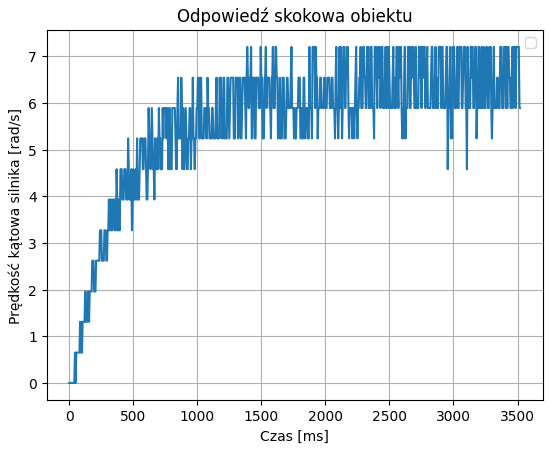
\includegraphics[width=12cm]{figures/PID/noreg.png}%
 \caption{Odpowiedź obiektu}%
 \label{Fig:noreg}%
\end{figure}

Aby dopasować odpowiedź obiektu do modelu transmitancji pierwszego rzędu, zastosowano metodę aproksymacji \cite{automatyka}. Polegała ona na dopasowaniu odpowiedniego modelu matematycznego do zebranych danych eksperymentalnych. W tym przypadku, model transmitancji pierwszego rzędu pozwolił na odpowiednie odwzorowanie zachowania obiektu w kontekście zmian sygnału sterującego. Dzięki temu można było przewidywać reakcję obiektu na różne zmiany sterowania.

\begin{lstlisting}[language=Python, caption=Kod aproksymujący odpowiedź, label={lst:fit1}]
import numpy as np
from scipy.optimize import curve_fit

time_step=5/1000
  
t = np.arange(0, len(actuals) * time_step, time_step)
odpowiedz_skokowa=actuals 

def first_order_transfer_function(t, K, T):
    return K * (1 - np.exp(-t / T))

popt, pcov = curve_fit(first_order_transfer_function, t, odpowiedz_skokowa)
K, T=popt

print("Wzmocnienie (K):", K)
print("Stala czasowa (T):", T)
\end{lstlisting}

Kod przedstawiony na listingu \ref{lst:fit1} służy do analizy danych eksperymentalnych reprezentujących odpowiedź skokową obiektu oraz aproksymowania tych danych do modelu transmitancji pierwszego rzędu. Najpierw tworzone są dane czasowe \textit{t}, a następnie dane odpowiedzi skokowej \textit{odpowiedz\_skokowa}. Definiowana jest funkcja \textit{first\_order\_transfer\_function}, która odpowiada transmitancji pierwszego rzędu. Następnie korzystając z funkcji \textit{curve\_fit} z biblioteki \textit{scipy.optimize}, dopasowywany jest model transmitancji pierwszego rzędu do danych odpowiedzi skokowej. Funkcja, jako wynik działania, zwraca wartość wzmocnienia \textit{K} oraz stałą czasową \textit{T}.

Rysunek \ref{Fig:aprox} ukazuje aproksymację modelu transmitancji pierwszego rzędu do danych pomiarowych. Wyznaczoną transmitancję obiektu opisuje wzór \ref{Eq:trans}.

\begin{equation}
G(s) = \frac{6.37}{1 + 0.44s}
\label{Eq:trans}
\end{equation}

\begin{figure}[ht]%
 \centering%
 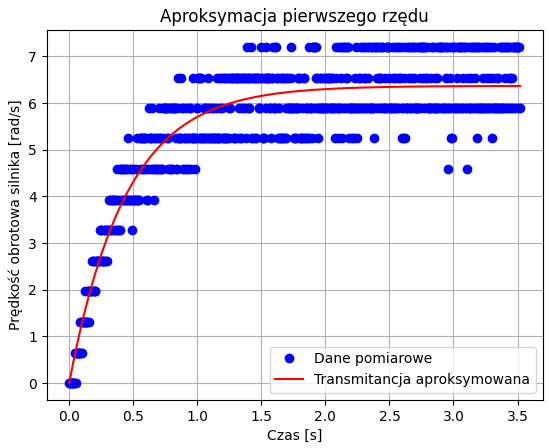
\includegraphics[width=12cm]{figures/PID/aprox.png}%
 \caption{Aproksymacja transmitancji}%
 \label{Fig:aprox}%
\end{figure}

\newpage

\subsubsection{Wyznaczenie nastaw metodą klasyczną}

Kod umieszczony na listingu \ref{lst:ziegler} wykorzystuje bibliotekę \textit{numpy} do obliczenia nastaw regulatora PID na podstawie zadanych wartości wzmocnienia i czasu wyprzedzenia. Na początku definiuje wartości stałych \textit{K} i \textit{T}, a następnie wykorzystuje je do obliczenia współczynnika krytycznego (\textit{Ku}) oraz okresu oscylacji (\textit{Tu}). Następnie na podstawie \textit{Ku} i \textit{Tu} wyznacza nastawy PID.

\begin{lstlisting}[caption={Kod z obliczeniami i wyświetleniem wyników}, label={lst:ziegler}]
import numpy as np

K = 6.365318519867311
T = 0.4425290896955204

Ku = 4 / (np.pi * K)

Tu = np.pi * T

Kp_PID = 0.20 * Ku
Ti_PID = 0.50 * Tu
Td_PID = 0.12 * Tu
\end{lstlisting}

\subsubsection{Algorytm genetyczny}

Optymalizacja nastaw regulatora PID jest kluczowym zagadnieniem w automatyce, które ma na celu poprawę wydajności systemów sterowania, w tym regulacji prędkości obrotowej silników. W kontekście fizycznego robota, możliwe jest utworzenie pętli uczącej, która będzie wprowadzać nowe współczynniki PID i testować je na rzeczywistym sprzęcie. Ogólny algorytm PID oraz komunikacja są obsługiwane przez oprogramowanie wgrane do mikrokontrolera robota. 

Z punktu widzenia automatyki, silnik prądu stałego jest stosunkowo prostym obiektem sterowania, co sprawia, że wiele zestawów parametrów może być odpowiednich do automatycznej regulacji prędkości. W związku z tym zdecydowano się na użycie algorytmu genetycznego do wyboru optymalnego zestawu współczynników PID.

Skrypt w języku Python zawierający implementację algorytmu genetycznego będzie uruchomiony na lokalnym serwerze. Każdy osobnik w populacji będzie testowany na fizycznym robocie w celu sprawdzenia jego dopasowania (\textit{fitness}). Algorytm będzie uruchamiany trzykrotnie z różnymi zestawami parametrów:

\begin{enumerate}[label=\alph*), leftmargin=1.25cm]
    \item \textbf{Pierwszy eksperyment}
    \begin{itemize}
        \item Rozmiar populacji: 100
        \item Maksymalna liczba epok: 25
        \item Prawdopodobieństwo krzyżowania: 70\%
        \item Liczba rodziców dla nowego osobnika: 10
        \item Prawdopodobieństwo mutacji: 15\%
    \end{itemize}
    
    \item \textbf{Drugi eksperyment}
    \begin{itemize}
        \item Rozmiar populacji: 200
        \item Maksymalna liczba epok: 25
        \item Prawdopodobieństwo krzyżowania: 70\%
        \item Liczba rodziców dla nowego osobnika: 15
        \item Prawdopodobieństwo mutacji: 15\%
    \end{itemize}
    
    \item \textbf{Trzeci eksperyment}
    \begin{itemize}
        \item Rozmiar populacji: 300
        \item Maksymalna liczba epok: 25
        \item Prawdopodobieństwo krzyżowania: 70\%
        \item Liczba rodziców dla nowego osobnika: 25
        \item Prawdopodobieństwo mutacji: 15\%
    \end{itemize}
\end{enumerate}


Ocena jakości regulacji będzie dokonywana na podstawie maksymalnego błędu regulacji, który docelowo musi być mniejszy lub równy 2\%. Algorytm zakończy swoje działanie po osiągnięciu maksymalnej liczby epok lub gdy zostanie spełniony warunek maksymalnego błędu regulacji.

Funkcja dopasowania, którą algorytm będzie maksymalizować, została określona jako odwrotność średniego błędu względnego (wzór \ref{Eq:fitness}) .

\begin{equation}
Fitness = \frac{1}{error}
\label{Eq:fitness}
\end{equation}

gdzie: $error$ - wartość średniego błędu względnego \\ \\

\newpage

\begin{lstlisting}[language=Python, caption=Konfiguracja MQTT, label={lst:genMQTT}]
import paho.mqtt.client as mqtt
import json
import time

MQTT_BROKER = "mqtt-dashboard.com"
MQTT_PORT = 1883
MQTT_TOPIC_PID = "robot/set/pid"
MQTT_TOPIC_MOTORS = "robot/set/motors"
MQTT_TOPIC_LOG = "robot/pid/log"
MQTT_TOPIC_RESPONSE = "robot/request"

mqtt_client = mqtt.Client("PID Ctl")

logs = []
experiment_ongoing = False

def on_log_message(client, userdata, message):
    global experiment_ongoing
    log_data = json.loads(message.payload.decode())
    if len(logs) != 0: 
        logs.append(log_data) 
    elif len(logs) == 0 and log_data["id"] == 0:
        logs.append(log_data)

def send_mqtt_message(topic, message):
    mqtt_client.publish(topic, json.dumps(message))
\end{lstlisting}

Kod przedstawiony na listingu \ref{lst:genMQTT} nawiązuje połączenie z brokerem MQTT, który umożliwia komunikację pomiędzy serwerem a robotem. Kluczowe elementy konfiguracji obejmują określenie adresu brokera oraz portu. Następnie zdefiniowano tematy MQTT do wysyłania i odbierania wiadomości dotyczących ustawień PID, sterowania silnikami oraz logowania. Dodatkowo zdefiniowano funkcje pomocnicze, takie jak \textit{send\_mqtt\_message} do wysyłania wiadomości oraz \textit{on\_log\_message} do obsługi wiadomości logowania.

Ta sekcja przedstawia funkcję \textit{run\_experiment} (listing \ref{lst:runExperiment}), która inicjalizuje i przeprowadza eksperymenty z nowymi nastawami PID na robocie. Kluczowe kroki obejmują ponowne połączenie z brokerem MQTT i subskrybowanie tematów logowania, wysłanie nowych wartości współczynników PID do robota, uruchomienie silników robota i monitorowanie ich przez określony czas oraz zbieranie danych logowania do późniejszej analizy.

\begin{lstlisting}[language=Python, caption=Funkcja uruchamiająca eksperyment, label={lst:runExperiment}]
def run_experiment(Kp, Ti, Td):
    global logs
    global mqtt_client
    global experiment_ongoing
    mqtt_client = mqtt.Client("PID ctl")
    mqtt_client.connect(MQTT_BROKER, MQTT_PORT)
    mqtt_client.subscribe(MQTT_TOPIC_LOG)
    mqtt_client.on_message = on_log_message

    mqtt_client.loop()
    logs = []

    pid_settings = {"Kp": Kp, "Ti": Ti, "Td": Td}
    send_mqtt_message(MQTT_TOPIC_PID, pid_settings)

    motors_speed = {"left": 0, "right": 50}
    send_mqtt_message(MQTT_TOPIC_MOTORS, motors_speed)
    experiment_ongoing = True
    start_time = time.time()
    while time.time() - start_time < 2:
        mqtt_client.loop()

    motors_speed = {"left": 0, "right": 0}
    send_mqtt_message(MQTT_TOPIC_MOTORS, motors_speed)

    start_time = time.time()

    while time.time() - start_time < 1:
        mqtt_client.loop()
    
    send_mqtt_message(MQTT_TOPIC_RESPONSE, "")
    experiment_ongoing = False
\end{lstlisting}

Funkcja \textit{calculate\_errors} (listing \ref{lst:calcErrors}) służy do obliczania błędów na podstawie danych logowania zebranych podczas eksperymentu. Kluczowe kroki obejmują obliczanie błędów absolutnych i względnych dla każdej próbki danych oraz obliczanie średniego błędu względnego, który jest używany jako miara jakości regulatora PID.

\begin{lstlisting}[language=Python, caption=Funkcja obliczająca błędy, label={lst:calcErrors}]
def calculate_errors(logs):
    absolute_errors = []
    relative_errors = []

    for i in range(len(logs)):
        measurement = logs[i]
        absolute_error = abs(measurement['target'] - measurement['actual'])
        
        if measurement['target'] != 0:
            relative_error = (absolute_error / measurement['target']) * 100
        else:
            if measurement['actual'] == measurement['target']:
                relative_error = 0
            else:
                relative_error = float(100)  
        
        absolute_errors.append(absolute_error)
        relative_errors.append(relative_error)

    mean_relative_error = (sum(relative_errors) / len(relative_errors)) if(len(relative_errors)) != 0 else 10000

    if(mean_relative_error) == 0.0:
        return 10000

    return mean_relative_error
\end{lstlisting}

Funkcja \textit{fitness\_func} (listing \ref{lst:fitnessFunc}) ocenia jakość każdego zestawu współczynników PID, wykonując eksperyment z tymi współczynnikami i obliczając wynikowy błąd względny. Wynik jest używany przez algorytm genetyczny do wyboru najlepszych rozwiązań. Kluczowe elementy obejmują przeprowadzenie eksperymentu z podanymi współczynnikami PID, wyliczenie średniego błędu względnego oraz zwrócenie wartości funkcji dopasowania, która jest odwrotnością błędu względnego.

\begin{lstlisting}[language=Python, caption=Funkcja dopasowania, label={lst:fitnessFunc}]
def fitness_func(ga_instance, solution, solution_idx):
    global logs
    global log_file

    Kp, Ti, Td = solution
    run_experiment(Kp, Ti, Td)

    mean_relative_error = calculate_errors(logs)
    logs = []
    append_data_to_csv(log_file, [Kp, Ti, Td, mean_relative_error, ga_instance.generations_completed])
    print(mean_relative_error)

    fitness = 1 / (mean_relative_error + 0.001)
    return fitness
\end{lstlisting}

Funkcja \textit{run\_genetic\_algorithm} (listing \ref{lst:runGA}) inicjalizuje i uruchamia algorytm genetyczny z podanymi parametrami. Kluczowe kroki obejmują definicję problemu optymalizacyjnego poprzez określenie liczby genów (współczynników PID) oraz przestrzeni poszukiwań, inicjalizację algorytmu genetycznego z parametrami takimi jak liczba pokoleń, liczba rodziców, prawdopodobieństwo krzyżowania i mutacji oraz wykonanie algorytmu i zapisanie najlepszego rozwiązania.

\begin{lstlisting}[language=Python, caption=Uruchamianie algorytmu genetycznego, label={lst:runGA}]
def run_genetic_algorithm(pop_size, max_epochs, crossover_prob, num_parents_mating, mutation_prob, experiment_num):
    num_genes = 3 

    on_generation = lambda x: save_best_solution(x, experiment_num)
    
    ga_instance = pygad.GA(num_generations=max_epochs,
                           num_parents_mating=num_parents_mating,
                           sol_per_pop=pop_size,
                           num_genes=num_genes,
                           gene_space={'low': 0, 'high': 30},
                           crossover_probability=crossover_prob,
                           mutation_percent_genes='default',
                           mutation_probability=mutation_prob,
                           K_tournament=num_parents_mating,
                           fitness_func=fitness_func,
                           on_generation=on_generation,
                           mutation_type='scramble',
                           crossover_type="uniform",
                           parent_selection_type='tournament',
                           keep_parents=0,
                           gene_type=float,
                           random_mutation_min_val=10,
                           random_mutation_max_val=20
                           )

    ga_instance.run()
    
    best_solution = ga_instance.best_solution()
    return best_solution
\end{lstlisting}

W tej sekcji (listing \ref{lst:experimentLoop}) kod inicjalizuje i przeprowadza serię eksperymentów z różnymi zestawami parametrów algorytmu genetycznego. Kluczowe kroki obejmują zdefiniowanie zestawów parametrów dla trzech różnych eksperymentów oraz iterację przez każdy zestaw parametrów, uruchamianie algorytmu genetycznego dla każdego z nich i zapisanie najlepszych rozwiązań.

\begin{lstlisting}[language=Python, caption=Pętla przeprowadzająca eksperymenty, label={lst:experimentLoop}]
experiments_params = [
    {"pop_size": 100, "max_epochs": 25, "crossover_prob": 0.70, "num_parents_mating": 10, "mutation_prob": 0.15},
    {"pop_size": 200, "max_epochs": 25, "crossover_prob": 0.70, "num_parents_mating": 15, "mutation_prob": 0.15},
    {"pop_size": 300, "max_epochs": 25, crossover_prob: 0.70, num_parents_mating: 20, mutation_prob: 0.15}
]

for i, params in enumerate(experiments_params):
    print(f"Starting experiment {i+1} with params: {params}")
    best_solution = run_genetic_algorithm(
        pop_size=params["pop_size"],
        max_epochs=params["max_epochs"],
        crossover_prob=params["crossover_prob"],
        num_parents_mating=params["num_parents_mating"],
        mutation_prob=params["mutation_prob"],
        experiment_num=i+1
    )
    print(f"Best solution for experiment {i+1}: {best_solution}")
\end{lstlisting}

\begin{figure}[ht]%
 \centering%
 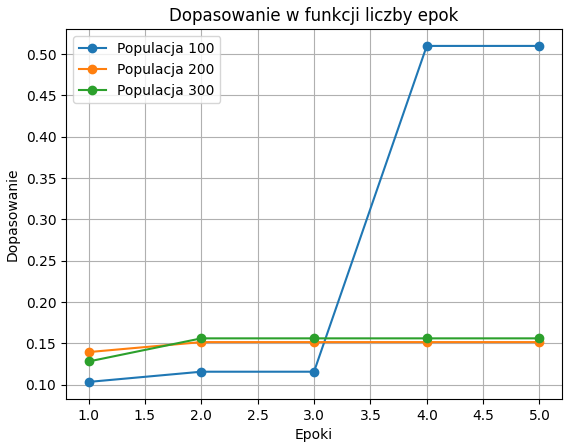
\includegraphics[width=10cm]{figures/PID/gen.png}%
 \caption{Dopasowanie w funkcji czasu}%
 \label{Fig:gen}%
\end{figure}

Uruchomienie tak przygotowanego skryptu pozwoliło na uzyskanie trzech zestawów nastaw regulatora PID. Rysunek \ref{Fig:gen} ukazuje dopasowanie najlepszego osobnika danej populacji w funkcji czasu (epok). Biorąc pod uwagę kształty wykresów, można dojśc do następującego wniosku: ze względu na prostotę obiektu, jakim jest silnik DC, wiele różnych od siebie zestawów nastaw regulatora jest w stanie usatysfakcjonować stawiane przed nim wymagania, przez co algorytm genetyczny popada w stagnację po osiągnięciu lokalnego minimum.



\subsubsection{Porównanie otrzymanych wyników}
Podczas przeprowadzania eksperymentu otrzymano następujące nastawy regulatora PID:

\begin{enumerate}[label=\alph*), leftmargin=1.25cm]
    \item \textbf{Ziegler-Nichols}
    \begin{itemize}
        \item Kp: 0.04
        \item Ti: 0.695
        \item Td: 0.166
    \end{itemize}
    
    \item \textbf{GA eksperyment 1}
    \begin{itemize}
        \item Kp: 6.48
        \item Ti: 2.93
        \item Td: 2.34
    \end{itemize}
    	
	\item \textbf{GA eksperyment 2}
    \begin{itemize}
        \item Kp: 29.50
        \item Ti: 14.54
        \item Td: 1.37
    \end{itemize}    	
    	
    	\item \textbf{GA eksperyment 3}
    \begin{itemize}
        \item Kp: 11.98
        \item Ti: 1.59
        \item Td: 1.34
    \end{itemize} 
    
\end{enumerate}
%
%
%
By porównać jakość wyznaczonych nastaw, należało przestroić regulator i zbadać odpowiedź obiektu na zmianę sygnału sterującego.
\begin{table}[ht]
\caption{Zestawienie wyników}
\centering		
	\begin{tabular}{|p{0.3\textwidth}|p{0.3\textwidth}|p{0.3\textwidth}|}	
		\hline
		Metoda & Czas ustalania [ms] & Uwagi \\
		\hline
		Ziegler-Nichols & 190 & Niedoregulowanie \\
		\hline
		GA eksperyment 1 & 630 & Niedoregulowanie \\
		\hline
		GA eksperyment 2 & 600 & Satysfakcjonująca regulacja \\
		\hline
		GA eksperyment 3 & 600 & Satysfakcjonująca regulacja \\
		\hline

	\end{tabular}	
	
\label{Tab:PID_comparision}
\end{table}	

\newpage

\begin{figure}[ht]%
 \centering%
 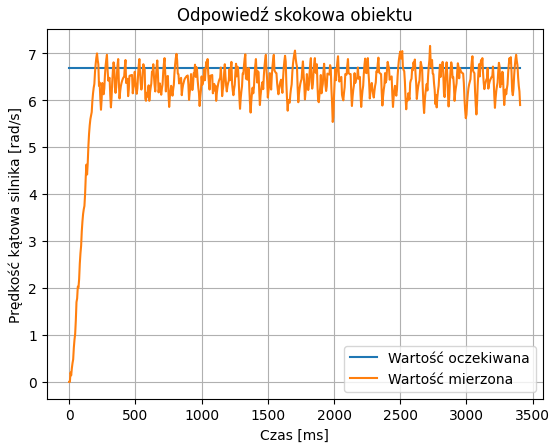
\includegraphics[width=10cm]{figures/PID/zieglerpid.png}%
 \caption{Nastawy wyznaczone metodą Zieglera-Nicholsa}%
 \label{Fig:zieglerpid}%
\end{figure}

\begin{figure}[ht]%
 \centering%
 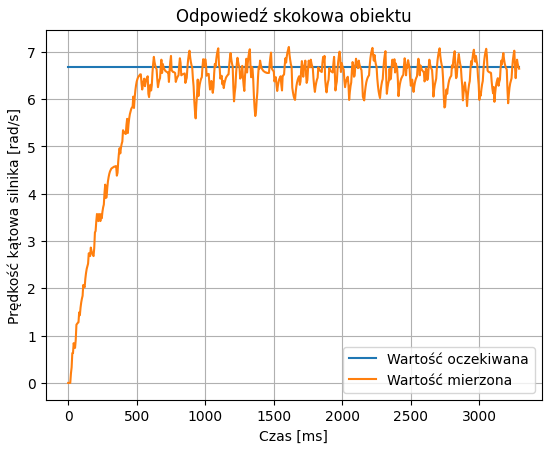
\includegraphics[width=10cm]{figures/PID/exp1pid.png}%
 \caption{Nastawy wyznaczone przez algorytm genetyczny (1)}%
 \label{Fig:exp1pid}%
\end{figure}

\begin{figure}[ht]%
 \centering%
 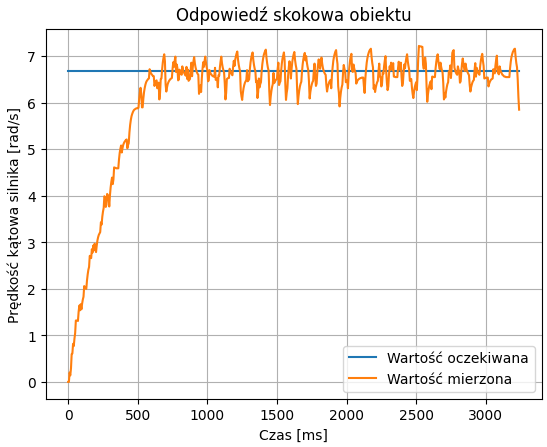
\includegraphics[width=10cm]{figures/PID/exp2pid.png}%
 \caption{Nastawy wyznaczone przez algorytm genetyczny (2)}%
 \label{Fig:exp2pid}%
\end{figure}

\begin{figure}[ht]%
 \centering%
 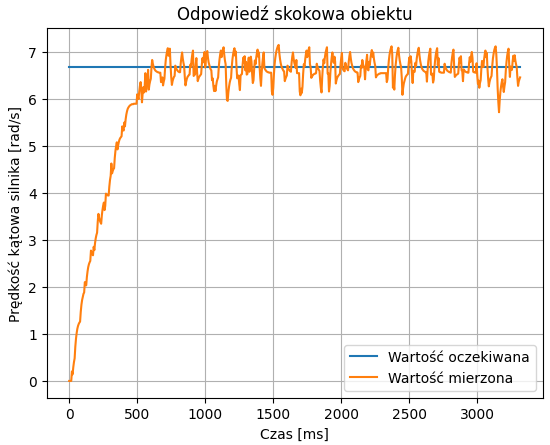
\includegraphics[width=10cm]{figures/PID/exp3pid.png}%
 \caption{Nastawy wyznaczone przez algorytm genetyczny (3)}%
 \label{Fig:exp3pid}%
\end{figure}

\clearpage

Po sprawdzeniu odpowiedzi obiektu na wyznaczone nastawy, podjęto decyzję o wykorzystaniu wyniku trzeciego eksperymentu. Wybór jest uzasadniony kilkoma kluczowymi czynnikami. Przede wszystkim, w porównaniu z innymi metodami, nastawy te zapewniły satysfakcjonującą regulację systemu (rysunek \ref{Fig:exp3pid}). Czas ustalania wynosił 600 ms, co jest wynikiem porównywalnym z najlepszymi nastawami uzyskanymi w innych eksperymentach. Dodatkowo, podczas eksperymentu nastawy GA 3 wykazały najlepszy wynik \textit{fitness}, co oznacza, że algorytm genetyczny skutecznie dostroił parametry regulatora w celu optymalnej regulacji systemu. W związku z tym, można uznać, że nastawy te są najkorzystniejsze pod względem jakości regulacji i efektywności działania systemu. Podczas testów z nastawami wyznaczonymi metodą Zieglera-Nicholsa (rysunek \ref{Fig:zieglerpid}) zaobserwowano, że jedno z kół nie chciało wystartować, co świadczy o niedostatecznej regulacji. Oznacza to, że te nastawy nie były w stanie zapewnić właściwej kontroli nad całym systemem, co może prowadzić do niestabilności i niesatysfakcjonującej wydajności. Czas ustalania wynoszący 190 ms jest krótki, ale ze względu na problem z jednym z kół, regulacja nie była wystarczająco dobra.



\subsection{Porównanie statycznych algorytmów nawigacyjnych w terenie bez przeszkód}
Niniejsza sekcja skupia się na opisie eksperymentu, który miał na celu porównanie wydajności algorytmu A* z różnymi heurystykami odległości (Manhattan, Euklidesowa, Max) oraz algorytmu Dijkstry na różnych rozmiarach grafów. Celem było zrozumienie, który algorytm lepiej nadaje się do rozwiązywania problemów przeszukiwania grafów w kontekście optymalizacji czasu działania i długości trasy, jaką ma pokonać robot. 



\subsubsection{Przebieg eksperymentu}
Mapa, po której przemieszczał się robot, to prostokąt o wymiarach 200x50 cm. Aby dokładnie ocenić efektywność algorytmów wyznaczania trasy, eksperyment uwzględnił kilka różnych rozmiarów map:

\begin{enumerate}[label=\alph*), leftmargin=1.25cm]
	\item oprócz podstawowej mapy o wymiarach 200x50 cm, przygotowano również mapy o większych rozmiarach: 200x200 cm, 500x500 cm, 1000x1000 cm oraz 2000x2000 cm,
	\item każda z tych map była reprezentowana jako graf, gdzie węzły odpowiadały punktom na mapie, a krawędzie określały możliwe połączenia między nimi.
	
\end{enumerate}

\begin{lstlisting}[caption={Porównanie algorytmów}, label={lst:staticAlgos}]
from graph_ops import load_graph_from_file
graph_dims = [(200, 50), (200, 200), (500, 500), (1000, 1000), (2000, 2000)]
graphs = {}

for dim in graph_dims:
    fname = f'graph_{dim[0]}_{dim[1]}.pkl'
    graphs[fname] = load_graph_from_file(fname)

start = (0, 0)
goal = (198, 40)

heuristics={
    "manhattan" : manhattan_distance,
    "euclidean" : euclidean_distance,
    "max" : max_distance
}

for k, v in heuristics.items():
    print(f"Funkcja obliczajaca odleglosc w algorytmie A*: {k}")
    for gname, graph in graphs.items():
        print(gname)
        path1 = a_star(graph, start, goal, v)
        path2 = dijkstra(graph, start, goal)
        print('\n')
\end{lstlisting}

Kod przedstawiony na listingu \ref{lst:staticAlgos} ukazuje skrypt odpowiedzialny za zbadanie algorytmów przeszukujących grafy. Kod rozpoczyna się od wczytania wcześniej wygenerowanych grafów i zdefiniowania heruystyk wykorzystanych w eksperymencie:

\begin{enumerate}[label=\alph*), leftmargin=1.25cm]
	\item Manhattan (wzór \ref{Eq:manhattan}),
	\item Euklidesowa (wzór \ref{Eq:euclidean}),
	\item Czebyszewa (wzór \ref{Eq:czebyszewa}).
	
\end{enumerate}

\begin{equation}
d_{\text{Manhattan}}(p, q) = |p_x - q_x| + |p_y - q_y|
\label{Eq:manhattan}
\end{equation}

\begin{equation}
d_{\text{Euklidesowa}}(p, q) = \sqrt{(p_x - q_x)^2 + (p_y - q_y)^2}
\label{Eq:euclidean}
\end{equation}

\begin{equation}
d_{\text{Czebyszewa}}(p, q) = \max(|p_x - q_x|, |p_y - q_y|)
\label{Eq:czebyszewa}
\end{equation}

gdzie: $p$, $q$ -- to punkty w dwuwymiarowej przestrzeni, gdzie każdy punkt jest reprezentowany przez parę współrzędnych $(p_x, p_y)$ i $(q_x, q_y)$, $d$ -- oznacza odległość pomiędzy punktem $p$ i $q$ \\

\newpage

Kolejnym krokiem jest przejście przez wszystkie heurystyki oraz wczytane grafy w celu przeprowadzenia eksperymentu porównawczego. Skrypt, dla każdego grafu, wyznacza trasę z punktu startowego \textit{start} do punktu docelowego \textit{goal} z wykorzystaniem określonej heurystyki.

\subsubsection{Porównanie otrzymanych wyników}

Na podstawie przedstawionych wyników eksperymentu porównującego algorytmy A* z różnymi heurystykami oraz algorytm Dijkstry (tabela \ref{Tab:comparison}), można wysunąć następujące wnioski:

\begin{enumerate}[label=\alph*), leftmargin=1.25cm]
	\item algorytm Dijkstry wypadł lepiej pod względem czasu wykonania w porównaniu do algorytmu A* (rysunek \ref{Fig:astar_vs_dijkstra}). Osiągnął on znacznie krótsze czasy wykonania dla wszystkich rozmiarów badanych grafów. Zwykle A* powinien działać szybciej, ponieważ używa heurystyki do prowadzenia wyszukiwania, co teoretycznie powinno ograniczyć liczbę odwiedzanych węzłów.
	\item heurystyka Manhattan osiągała najkrótsze czasy wykonania dla większości badanych przypadków jednocześnie minimalnie odstając od pozostałych. W bardziej złożonym środowisku może to prowadzić do oszczędności czasu, ponieważ odległość manhattańska jest obliczeniowo najmniej złożoną heurystyką spośród badanych.
\end{enumerate}

\begin{figure}[ht]%
 \centering%
 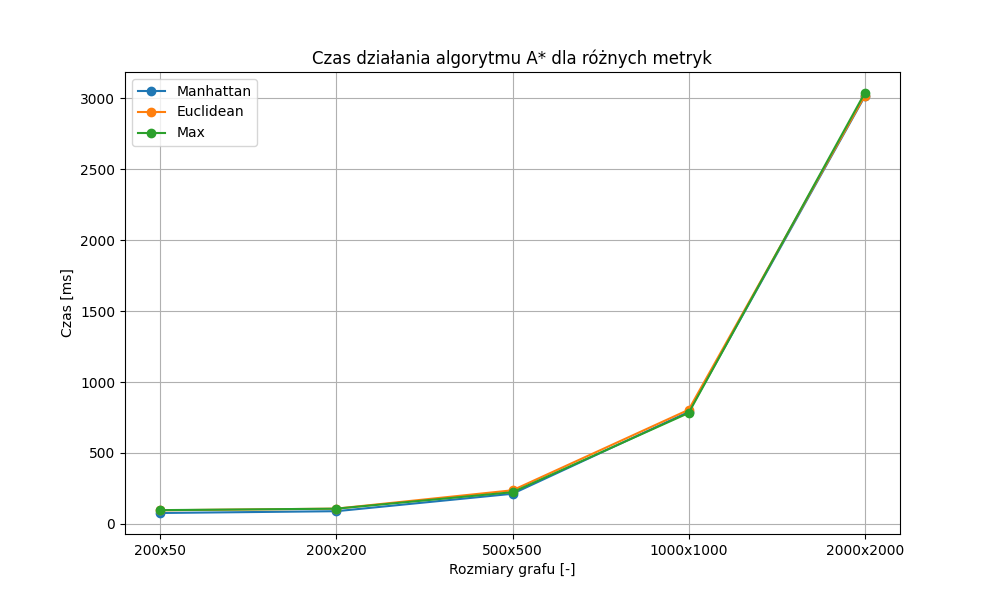
\includegraphics[width=12cm]{figures/static_algo/charts/nowalls/astar_heuristics.png}%
 \caption{Czas działania algorytmu A*}%
 \label{Fig:astar_heuristics}%
\end{figure}

\begin{figure}[ht]%
 \centering%
 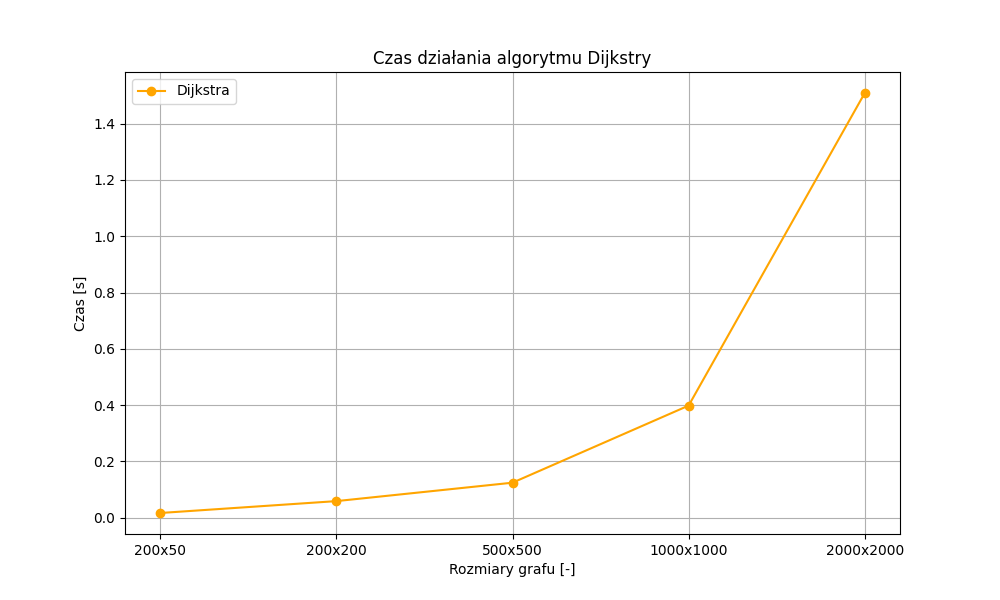
\includegraphics[width=12cm]{figures/static_algo/charts/nowalls/dijkstra.png}%
 \caption{Czas działania algorytmu Dijkstry}%
 \label{Fig:dijkstra}%
\end{figure}

\begin{figure}[ht]%
 \centering%
 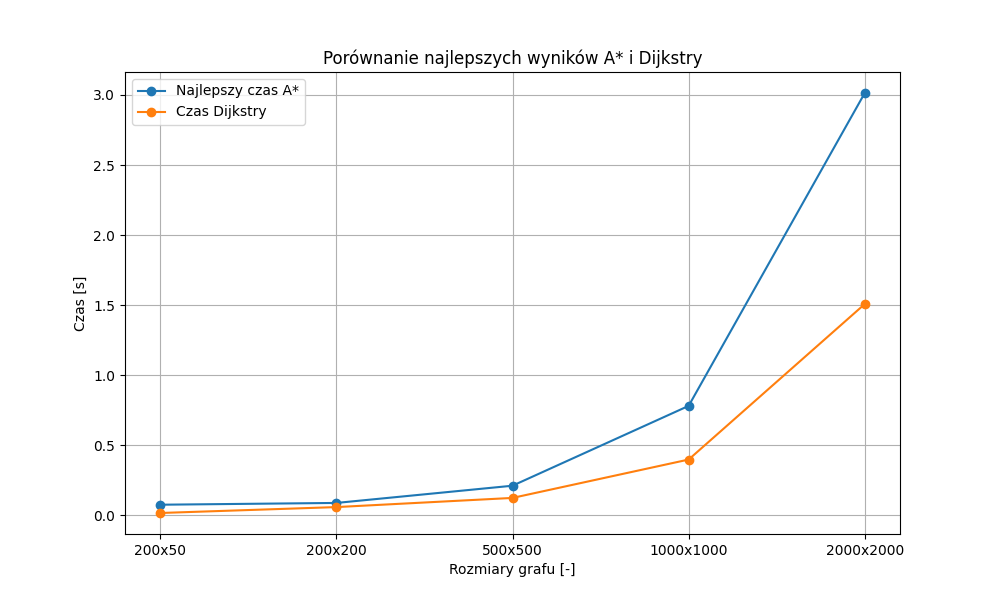
\includegraphics[width=12cm]{figures/static_algo/charts/nowalls/astar_vs_dijkstra.png}%
 \caption{Porównanie czasu działania algorytmów}%
 \label{Fig:astar_vs_dijkstra}%
\end{figure}

\clearpage

\begin{table}[ht]
\caption{Wyniki algorytmu A* dla różnych heurystyk}
\centering		
\begin{tabular}{|p{0.3\textwidth}|p{0.3\textwidth}|p{0.3\textwidth}|}	
\hline
Heurystyka & Graf & Czas [ms] \\
\hline
Manhattan & 
graph\_200\_50.pkl & 
76.2 \\
 & 
graph\_200\_200.pkl & 
88.9 \\
 & 
graph\_500\_500.pkl & 
211.8 \\
 & 
graph\_1000\_1000.pkl & 
789.2 \\
 & 
graph\_2000\_2000.pkl & 
3014.2 \\
\hline
Euclidean & 
graph\_200\_50.pkl & 
95.2 \\
 & 
graph\_200\_200.pkl & 
107.0 \\
 & 
graph\_500\_500.pkl & 
236.4 \\
 & 
graph\_1000\_1000.pkl & 
804.1 \\
 & 
graph\_2000\_2000.pkl & 
3019.3 \\
\hline
Max & 
graph\_200\_50.pkl & 
96.4 \\
 & 
graph\_200\_200.pkl & 
106.7 \\
 & 
graph\_500\_500.pkl & 
222.9 \\
 & 
graph\_1000\_1000.pkl & 
781.5 \\
 & 
graph\_2000\_2000.pkl & 
3038.1 \\
\hline
\end{tabular}	

\label{Tab:Astar_results}
\end{table}



\begin{table}[ht]
\caption{Wyniki algorytmu Dijkstry}
\centering		
\begin{tabular}{|p{0.5\textwidth}|p{0.4\textwidth}|}	
\hline
Graf & Czas [ms] \\
\hline
graph\_200\_50.pkl & 
17.1 \\
graph\_200\_200.pkl & 
59.3 \\
graph\_500\_500.pkl & 
124.7 \\
graph\_1000\_1000.pkl & 
398.5 \\
graph\_2000\_2000.pkl & 
1508.4 \\
\hline
\end{tabular}	

\label{Tab:Dijkstra_results}
\end{table}


\begin{table}[ht]
\caption{Tabela porównawcza najlepszych wyników A* i Dijkstry}
\centering		
\begin{tabular}{|p{0.3\textwidth}|p{0.3\textwidth}|p{0.3\textwidth}|}	
\hline
Graf & Najlepszy czas A* [ms] & Czas Dijkstry [ms] \\
\hline
graph\_200\_50.pkl & 
76.2 & 
17.1 \\
graph\_200\_200.pkl & 
88.9 & 
59.3 \\
graph\_500\_500.pkl & 
211.8 & 
124.7 \\
graph\_1000\_1000.pkl & 
781.5 & 
398.5 \\
graph\_2000\_2000.pkl & 
3014.2 & 
1508.4 \\
\hline
\end{tabular}	

\label{Tab:comparison}
\end{table}

\clearpage

\subsection{Porównanie statycznych algorytmów nawigacyjnych w terenie z przeszkodami}

W niniejszej sekcji przedstawiono opis eksperymentu, który rozszerza badanie efektywności algorytmów A* z różnymi heurystykami oraz algorytmu Dijkstry na teren z przeszkodami. Celem eksperymentu było porównanie, który z tych algorytmów lepiej radzi sobie ze znajdowaniem najkrótszej trasy w grafach reprezentujących mapę z przeszkodami. Dodatkowo, oprócz optymalizacji czasu działania, analizowano zdolność algorytmów do efektywnego omijania przeszkód i wyznaczania tras optymalnych pod względem długości. Eksperyment ten ma na celu dostarczenie danych na temat wyboru odpowiedniego algorytmu nawigacyjnego w różnych warunkach terenowych.

\subsubsection{Przebieg eksperymentu}

W celu porównania wydajności różnych heurystyk oraz algorytmu Dijkstry w kontekście znajdowania najkrótszej ścieżki w grafach reprezentujących mapy z przeszkodami, przeprowadzono serię eksperymentów. Każdy eksperyment składał się z następujących kroków:

\begin{enumerate}[label=\alph*), leftmargin=1.25cm]
    \item wygenerowanie siatki grafu o wymiarach 200x50,
    \item losowe dodanie 130 przeszkód o różnych rozmiarach,
    \item określenie punktu startowego oraz celu na mapie,
    \item przeprowadzenie procesu wyszukiwania najkrótszej ścieżki za pomocą algorytmu A* i Dijkstry,
    \item pomiar długości znalezionych ścieżek i porównanie efektywności obu algorytmów.
\end{enumerate}

Każdy z eksperymentów został powtórzony pięciokrotnie w celu uzyskania średnich wyników oraz zapewnienia wiarygodności otrzymanych danych. Wyniki eksperymentów zostały szczegółowo udokumentowane, prezentując zarówno długości ścieżek uzyskane przez każdy z algorytmów, jak i wizualizacje zaznaczające przebieg tych ścieżek na mapie. Eksperymenty te miały na celu nie tylko zidentyfikowanie najbardziej efektywnego algorytmu w kontekście czasu obliczeń, ale również ocenę ich zdolności do omijania przeszkód oraz znajdowania optymalnych tras na mapach złożonych z różnorodnych przeszkód. Dokładny przebieg eksperymentu został przedstawiony na listingu \ref{lst:experimentStatic}.


\begin{lstlisting}[language=Python, caption={Porównanie algorytmów}, label={lst:experimentStatic}]
for i in range(5):
    graph = create_grid_graph(200, 50)
    add_random_obstacles(graph, 130, 10, 10)

    draw_map(graph, None, f'map_{i}.png')


    start = (0, 30)
    goal = (199, 20)

    heuristics={
        "manhattan" : manhattan_distance,
        "euclidean" : euclidean_distance,
        "max" : max_distance
    }

    print(f"iteracja: {i}")
    path2 = dijkstra(graph, start, goal)
    print(f"Dlugosc trasy Dijkstra: {calculate_path_length(path2)}")
    draw_map(graph, path2, f'map_dijkstra_{i}.png')


    for k, v in heuristics.items():
        print(f"Funkcja obliczajaca odleglosc w algorytmie A*: {k}")
        path1 = a_star(graph, start, goal, v)
        print(f"Dlugosc trasy A*: {calculate_path_length(path1)}, { k }")
        draw_map(graph, path1, f'map_astar_{k}_{i}.png')
\end{lstlisting}

\newpage

\subsubsection{Porównanie otrzymanych wyników}

Podsumowanie wyników przedstawionych w tabeli \ref{Tab:Astar_Dijkstra_results} wskazuje, że algorytm Dijkstry osiągnął najlepsze wyniki pod względem czasu działania dla wszystkich iteracji, utrzymując przy tym identyczną długość wyznaczonej trasy (247 dla iteracji 0, 1, 2, 4 oraz 233 dla iteracji 3). Algorytmy A* z różnymi heurystykami uzyskały takie same wyniki pod względem długości trasy, jednak wymagały więcej czasu obliczeniowego w porównaniu do Dijkstry (rysunek \ref{Fig:astar_vs_dijkstra_walls}).

\begin{table}[h]
\centering
\begin{tabular}{|p{0.1\textwidth}|p{0.25\textwidth}|p{0.25\textwidth}|p{0.25\textwidth}|}    
\hline
\textbf{Iteracja} & \textbf{Algorytm} & \textbf{Czas działania algorytmu [ms]} & \textbf{Długość trasy} \\
\hline
0 & 
A* Manhattan & 
114.0 & 
247 \\
 & 
A* Euclidean & 
103.0 & 
247 \\
 & 
A* Max & 
99.1 & 
247 \\
 & 
Dijkstra & 
23.4 & 
247 \\
\hline
1 & 
A* Manhattan & 
103.0 & 
243 \\
 & 
A* Euclidean & 
121.6 & 
243 \\
 & 
A* Max & 
119.7 & 
243 \\
 & 
Dijkstra & 
16.9 & 
243 \\
\hline
2 & 
A* Manhattan & 
122.4 & 
247 \\
 & 
A* Euclidean & 
130.9 & 
247 \\
 & 
A* Max & 
142.5 & 
247 \\
 & 
Dijkstra & 
18.7 & 
247 \\
\hline
3 & 
A* Manhattan & 
56.8 & 
233 \\
 & 
A* Euclidean & 
104.8 & 
233 \\
 & 
A* Max & 
102.0 & 
233 \\
 & 
Dijkstra & 
18.4 & 
233 \\
\hline
4 & 
A* Manhattan & 
85.4 & 
243 \\
 & 
A* Euclidean & 
92.3 & 
243 \\
 & 
A* Max & 
98.4 & 
243 \\
 & 
Dijkstra & 
18.2 & 
243 \\
\hline
\end{tabular}
\caption{Porównanie czasu działania i długości trasy dla algorytmu A* z różnymi heurystykami oraz algorytmu Dijkstry}
\label{Tab:Astar_Dijkstra_results}
\end{table}


\begin{figure}[ht]%
 \centering%
 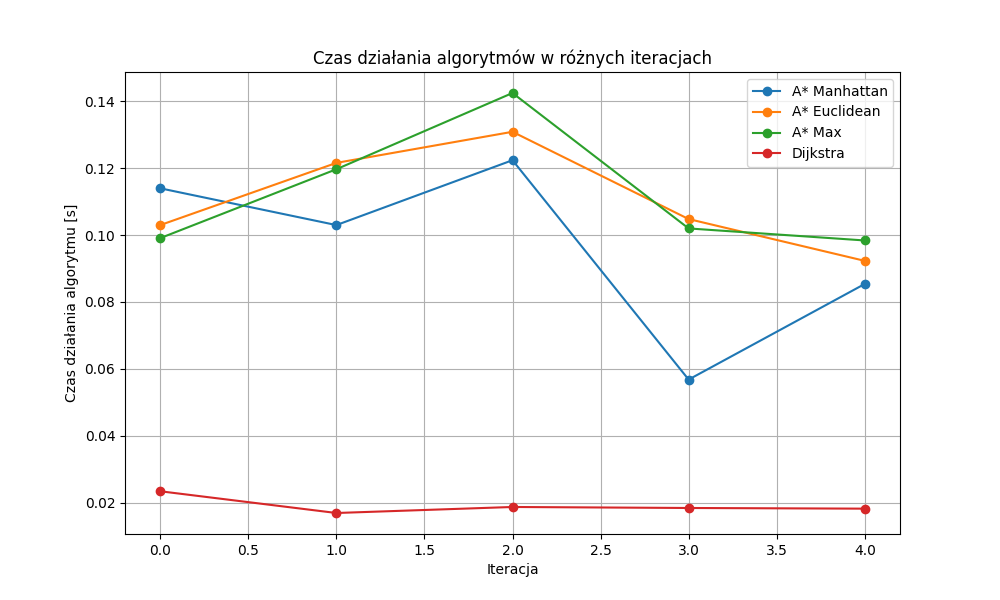
\includegraphics[width=12cm]{figures/static_algo/charts/walls/algorithm_times_walls.png}%
 \caption{Porównanie czasu działania algorytmów}%
 \label{Fig:astar_vs_dijkstra_walls}%
\end{figure}

Na niżej ukazanych obrazkach przedstawiono wyniki działania algorytmów przeszukiwania grafu dla dwóch wybranych iteracji. Każdy zestaw obrazków składa się z dwóch głównych sekcji: mapy ogólnej, porównania ścieżek dla algorytmów A* z różnymi heurystykami oraz algorytmu Dijkstry.


%% Iteracja 0
%\begin{figure}[ht]
%    \centering
%    
\includegraphics[width=0.6\textwidth]{figures/static_algo/map_0.png}
%    \caption{Mapa dla iteracji 0}
%    \label{fig:map_0}
%\end{figure}
%
%\begin{figure}[ht]
%    \centering
%    \begin{minipage}{0.4\textwidth}
%        \centering
%        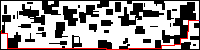
\includegraphics[width=\linewidth]{figures/static_algo/map_astar_manhattan_0.png}
%        \caption*{A* z heurystyką Manhattan}
%        \label{fig:map_astar_manhattan_0}
%    \end{minipage}
%    \hspace{0.1\textwidth}
%    \begin{minipage}{0.4\textwidth}
%        \centering
%        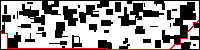
\includegraphics[width=\linewidth]{figures/static_algo/map_astar_euclidean_0.png}
%        \caption*{A* z heurystyką Euklidesową}
%        \label{fig:map_astar_euclidean_0}
%    \end{minipage}
%    \vspace{0.5cm}
%    
%	\begin{minipage}{0.4\textwidth}
%        \centering
%        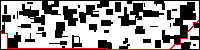
\includegraphics[width=\linewidth]{figures/static_algo/map_astar_max_0.png}
%        \caption*{Max}
%        \label{fig:map_astar_max_0}
%    \end{minipage}    
%    \hspace{0.1\textwidth}
%    \begin{minipage}{0.4\textwidth}
%        \centering
%        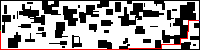
\includegraphics[width=\linewidth]{figures/static_algo/map_dijkstra_0.png}
%        \caption*{Dijkstra}
%        \label{fig:map_dijkstra_0}
%    \end{minipage}
%    \caption{Porównanie wyznaczonych ścieżek dla iteracji 0}
%    \label{fig:comparison_iteration_0}
%\end{figure}
%
%\clearpage

%% Iteracja 1
%\begin{figure}[ht]
%    \centering
%    
\includegraphics[width=0.6\textwidth]{figures/static_algo/map_1.png}
%    \caption{Mapa dla iteracji 1}
%    \label{fig:map_0}
%\end{figure}
%
%\begin{figure}[ht]
%    \centering
%    \begin{minipage}{0.4\textwidth}
%        \centering
%        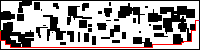
\includegraphics[width=\linewidth]{figures/static_algo/map_astar_manhattan_1.png}
%        \caption*{A* z heurystyką Manhattan}
%        \label{fig:map_astar_manhattan_1}
%    \end{minipage}
%    \hspace{0.1\textwidth}
%    \begin{minipage}{0.4\textwidth}
%        \centering
%        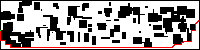
\includegraphics[width=\linewidth]{figures/static_algo/map_astar_euclidean_1.png}
%        \caption*{A* z heurystyką Euklidesową}
%        \label{fig:map_astar_euclidean_1}
%    \end{minipage}
%    \vspace{0.5cm}
%    
%	\begin{minipage}{0.4\textwidth}
%        \centering
%        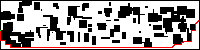
\includegraphics[width=\linewidth]{figures/static_algo/map_astar_max_1.png}
%        \caption*{Max}
%        \label{fig:map_astar_max_1}
%    \end{minipage}    
%    \hspace{0.1\textwidth}
%    \begin{minipage}{0.4\textwidth}
%        \centering
%        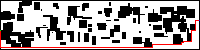
\includegraphics[width=\linewidth]{figures/static_algo/map_dijkstra_1.png}
%        \caption*{Dijkstra}
%        \label{fig:map_dijkstra_1}
%    \end{minipage}
%    \caption{Porównanie wyznaczonych ścieżek dla iteracji 1}
%    \label{fig:comparison_iteration_1}
%\end{figure}

%% Iteracja 2
%\begin{figure}[ht]
%    \centering
%    
\includegraphics[width=0.6\textwidth]{figures/static_algo/map_2.png}
%    \caption{Mapa dla iteracji 2}
%    \label{fig:map_2}
%\end{figure}
%
%\begin{figure}[ht]
%    \centering
%    \begin{minipage}{0.4\textwidth}
%        \centering
%        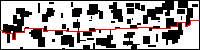
\includegraphics[width=\linewidth]{figures/static_algo/map_astar_manhattan_2.png}
%        \caption*{A* z heurystyką Manhattan}
%        \label{fig:map_astar_manhattan_2}
%    \end{minipage}
%    \hspace{0.1\textwidth}
%    \begin{minipage}{0.4\textwidth}
%        \centering
%        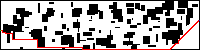
\includegraphics[width=\linewidth]{figures/static_algo/map_astar_euclidean_2.png}
%        \caption*{A* z heurystyką Euklidesową}
%        \label{fig:map_astar_euclidean_2}
%    \end{minipage}
%    \vspace{0.5cm}
%    
%	\begin{minipage}{0.4\textwidth}
%        \centering
%        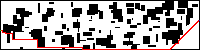
\includegraphics[width=\linewidth]{figures/static_algo/map_astar_max_2.png}
%        \caption*{Max}
%        \label{fig:map_astar_max_2}
%    \end{minipage}    
%    \hspace{0.1\textwidth}
%    \begin{minipage}{0.4\textwidth}
%        \centering
%        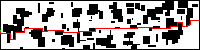
\includegraphics[width=\linewidth]{figures/static_algo/map_dijkstra_2.png}
%        \caption*{Dijkstra}
%        \label{fig:map_dijkstra_2}
%    \end{minipage}
%    \caption{Porównanie wyznaczonych ścieżek dla iteracji 2}
%    \label{fig:comparison_iteration_2}
%\end{figure}

% Iteracja 3
\begin{figure}[ht]
    \centering
    
\includegraphics[width=0.6\textwidth]{figures/static_algo/map_3.png}
    \caption{Mapa dla iteracji 3}
    \label{fig:map_3}
\end{figure}

\begin{figure}[ht]
    \centering
    \begin{minipage}{0.4\textwidth}
        \centering
        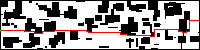
\includegraphics[width=\linewidth]{figures/static_algo/map_astar_manhattan_3.png}
        \caption*{A* z heurystyką Manhattan}
        \label{fig:map_astar_manhattan_3}
    \end{minipage}
    \hspace{0.1\textwidth}
    \begin{minipage}{0.4\textwidth}
        \centering
        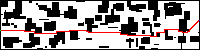
\includegraphics[width=\linewidth]{figures/static_algo/map_astar_euclidean_3.png}
        \caption*{A* z heurystyką Euklidesową}
        \label{fig:map_astar_euclidean_3}
    \end{minipage}
    \vspace{0.5cm}
    
	\begin{minipage}{0.4\textwidth}
        \centering
        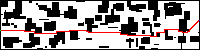
\includegraphics[width=\linewidth]{figures/static_algo/map_astar_max_3.png}
        \caption*{Max}
        \label{fig:map_astar_max_3}
    \end{minipage}    
    \hspace{0.1\textwidth}
    \begin{minipage}{0.4\textwidth}
        \centering
        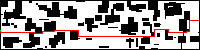
\includegraphics[width=\linewidth]{figures/static_algo/map_dijkstra_3.png}
        \caption*{Dijkstra}
        \label{fig:map_dijkstra_3}
    \end{minipage}
    \caption{Porównanie wyznaczonych ścieżek dla iteracji 3}
    \label{fig:comparison_iteration_3}
\end{figure}
\clearpage
%
% Iteracja 4
\begin{figure}[ht]
    \centering
    
\includegraphics[width=0.6\textwidth]{figures/static_algo/map_4.png}
    \caption{Mapa dla iteracji 4}
    \label{fig:map_4}
\end{figure}

\begin{figure}[ht]
    \centering
    \begin{minipage}{0.4\textwidth}
        \centering
        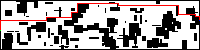
\includegraphics[width=\linewidth]{figures/static_algo/map_astar_manhattan_4.png}
        \caption*{A* z heurystyką Manhattan}
        \label{fig:map_astar_manhattan_4}
    \end{minipage}
    \hspace{0.1\textwidth}
    \begin{minipage}{0.4\textwidth}
        \centering
        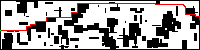
\includegraphics[width=\linewidth]{figures/static_algo/map_astar_euclidean_4.png}
        \caption*{A* z heurystyką Euklidesową}
        \label{fig:map_astar_euclidean_4}
    \end{minipage}
    \vspace{0.5cm}
    
	\begin{minipage}{0.4\textwidth}
        \centering
        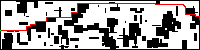
\includegraphics[width=\linewidth]{figures/static_algo/map_astar_max_4.png}
        \caption*{Max}
        \label{fig:map_astar_max_4}
    \end{minipage}    
    \hspace{0.1\textwidth}
    \begin{minipage}{0.4\textwidth}
        \centering
        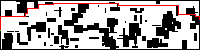
\includegraphics[width=\linewidth]{figures/static_algo/map_dijkstra_4.png}
        \caption*{Dijkstra}
        \label{fig:map_dijkstra_4}
    \end{minipage}
    \caption{Porównanie wyznaczonych ścieżek dla iteracji 4}
    \label{fig:comparison_iteration_4}
\end{figure}
%
%\clearpage

\subsection{Porównanie dynamicznych algorytmów nawigacyjnych w terenie z przeszkodami}
Niniejsza sekcja koncentruje się na opisie przeprowadzonego eksperymentu mającego na celu porównanie efektywności dwóch dynamicznych algorytmów nawigacyjnych: D* oraz D* Lite. Głównym celem badania jest ocena, który z tych algorytmów lepiej radzi sobie z nawigacją we wcześniej nieznanym środowisku, które może zawierać przeszkody.

\subsubsection{Przebieg eksperymentu}
Eksperyment skoncentrował się na porównaniu dwóch dynamicznych algorytmów nawigacyjnych: D* i D* Lite z algorytmem A* z metryką Manhattan słżącym jako algorytm bazowy. Badanie miało na celu ocenę, który z algorytmów dynamicznych lepiej radzi sobie z adaptacją do zmieniającego się środowiska oraz efektywnością znajdowania optymalnych ścieżek w terenie z przeszkodami. W każdej iteracji eksperymentu wykorzystano mapę o rozmiarach 100x100 cm z wyznaczonymi punktami startowymi i celowymi. Następnie, w zależności od iteracji, zmieniano rozmieszczenie i liczbę przeszkód w środowisku, po którym poruszał się robot.

Algorytmy testowane były na tej samej mapie, tych samych punktach startowych i docelowych. Po wykryciu przeszkody, każdy z algorytmów rozpoczynał proces wyznaczania ścieżki od nowa, biorąc pod uwagę aktualne warunki terenowe.

\subsubsection{Porównanie otrzymanych wyników}
Na podstawie danych przedstawionych w tabeli \ref{tab:dstar_vs_dstarlite} można wysunąć następujące wnioski:

\begin{enumerate}[label=\alph*), leftmargin=1.25cm]
    \item w przypadku wszystkich scenariuszy, algorytm D* Lite wykazał się minimalnie lepszym czasem działania w porównaniu do D* (rysunek \ref{Fig:dstar_vs_lite}). Taki wynik może być spowodowany tym, że w badanych scenariuszach występowała stosunkowo mała ilość napotkanych przeszkód oraz mapa była małych rozmiarów, co ograniczało liczbę operacji wymaganych do znalezienia optymalnej ścieżki,
    \item robot pokonał praktycznie tę samą odległość w każdym z pięciu przeprowadzonych scenariuszy testowych. Z uwagi na minimalnie lepszy czas działania, jaki uzyskał algorytm D* Lite, warto zdecydować się na jego wybór, szczególnie w kontekście optymalizacji czasu obliczeń w bardziej wymagających środowiskach. 
\end{enumerate}

\begin{figure}[ht]%
 \centering%
 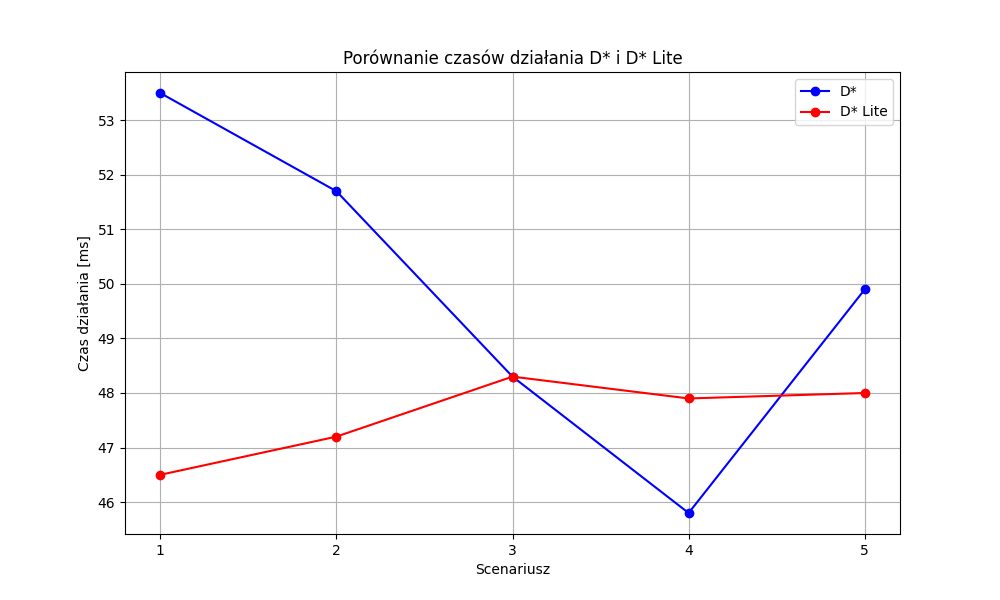
\includegraphics[width=12cm]{figures/dynamic/dstar_vs_lite.png}%
 \caption{Porównanie czasu działania algorytmów}%
 \label{Fig:dstar_vs_lite}%
\end{figure}

\begin{table}[h]
\centering
\begin{tabular}{|p{0.2\textwidth}|p{0.2\textwidth}|p{0.2\textwidth}|p{0.2\textwidth}|}
\hline
Iteracja & Ilość przeszkód & Czas działania dstar [ms], Pokonana odległość & Czas działania dstar\_lite [ms], Pokonana odległość \\
\hline
1 & 4 &
53.5, 112 & 
46.5, 112 \\
\hline
2 & 4 &
51.7, 105 & 
47.2, 105 \\
\hline
3 & 0 &
48.3, 101 & 
48.3, 101 \\
\hline
4 & 3 &
45.8, 106 & 
47.9, 107 \\
\hline
5 & 2 &
49.9, 115 & 
48.0, 115 \\
\hline
\end{tabular}
\caption{Porównanie czasów działania i pokonanych odległości dla D* i D* Lite}
\label{tab:dstar_vs_dstarlite}
\end{table}




\section{Podsumowanie i wnioski końcowe}
W niniejszym rozdziale przedstawiono podsumowanie oraz wnioski końcowe wynikające z przeprowadzonych eksperymentów dotyczących optymalizacji nastaw regulatora PID oraz porównania różnych algorytmów statycznych i dynamicznych w kontekście nawigacji.

\subsection{Optymalizacja nastaw regulatora PID}
Podczas badań nad optymalizacją nastaw regulatora PID przeprowadzono szereg eksperymentów, których celem było znalezienie optymalnych parametrów regulacji. W szczególności, eksperyment z algorytmem genetycznym (GA 3) wykazał się najbardziej satysfakcjonującymi wynikami pod względem jakości regulacji oraz czasu ustalania. Nastawy te charakteryzowały się czasem ustalania na poziomie 600 ms, co jest akceptowalnym wynikiem w porównaniu do innych eksperymentów. W przeciwieństwie do tego, próby z nastawami metodą Zieglera-Nicholsa nie zapewniły odpowiedniej stabilności, co objawiało się problemami z działaniem jednego z elementów systemu.

Podsumowując, najlepszym wyborem okazały się nastawy uzyskane z algorytmu genetycznego (GA 3), ze względu na skuteczność w regulacji systemu.

\subsection{Porównanie statycznych algorytmów nawigacyjnych w terenie bez przeszkód}
Analizując wyniki eksperymentu porównującego algorytmy A* z różnymi heurystykami oraz algorytm Dijkstry, można wysunąć kilka istotnych wniosków. Algorytm Dijkstry osiągnął znacznie lepsze czasy wykonania w porównaniu do A*, co może być zaskakującym wynikiem, biorąc pod uwagę, że A* powinien działać szybciej. Heurystyka Manhattan wykazała się jako najbardziej efektywna pod względem szybkości obliczeń, co czyni ją najlepszym wyborem dla tego konkretnego eksperymentu.

Podsumowując, algorytm Dijkstry był najbardziej efektywny pod względem czasu wykonania i powinien być preferowany w przypadku prostych zastosowań nawigacyjnych bez przeszkód.

\subsection{Porównanie statycznych algorytmów nawigacyjnych w terenie z przeszkodami}
Eksperymenty porównujące algorytmy A* z Dijkstrą w obecności przeszkód potwierdziły, że algorytm Dijkstry nadal był najbardziej efektywny pod względem czasu działania, przy jednoczesnym utrzymaniu identycznej długości wyznaczonej trasy. Wyniki te sugerują, że pomimo zastosowania różnych heurystyk w algorytmie A*, jego wydajność nadal była gorsza niż prosty algorytm Dijkstry w kontekście nawigacji w złożonym środowisku.

Podsumowując, algorytm Dijkstry może być zaimplementowany do zastosowań nawigacyjnych w prostych środowiskach z przeszkodami, zapewniając zarówno efektywność czasową, jak i optymalizację długości trasy.

\subsection{Porównanie dynamicznych algorytmów nawigacyjnych w terenie z przeszkodami}
Badania porównawcze algorytmów D* i D* Lite w różnych scenariuszach wykazały, że D* Lite osiąga nieznacznie lepsze czasy wykonania. Prawdopodobnie jest to rezultat mniejszej liczby przeszkód oraz mniejszej skali badanych map. Pomimo minimalnej różnicy w czasie działania, algorytm D* Lite wydaje się być bardziej efektywnym rozwiązaniem do zastosowań w bardziej wymagających środowiskach nawigacyjnych.

Podsumowując, ze względu lepszą efektywność czasową i potencjał do skutecznego działania w złożonych scenariuszach nawigacyjnych, algorytm D* Lite może być preferowany jako rozwiązanie problemu nawigacyjnego.

\subsection{Wkład własny}
Za wkład własny autor uważa:
\begin{enumerate}[label=\alph*), leftmargin=1.25cm]
\item projekt, implementację oraz testy elektroniki i oprogramowania robota zgodnie z procedurami ASPICE,
\item fizyczną realizację konstrukcji robota,
\item implementację skryptów niezbędnych do przeprowadzenia opisanych w tej pracy badań,
\item przeprowadzenie badań, obróbka danych i analiza wyników.
\end{enumerate}


\clearpage

\addcontentsline{toc}{section}{Literatura}

\begin{thebibliography}{15}
\bibitem{repo}Repozytorium z projektem: https://github.com/DevxMike/master\_degree

\bibitem{deepLearning} Francois Chollet: Deep Learning. Praca z językiem Python i biblioteką Keras. Helion 2019

\bibitem{cpp} Bjarne Stroustrup: The C++ Programming Language. Addison-Wesley Professional 2013

\bibitem{RL} Paweł Cichosz: Systemy uczące się. WNT 2007 

\bibitem{freeRTOS} Warren Gay: FreeRTOS for ESP32-Arduino. Elektor International Media b.v. 2020

\bibitem{genetics}  Riccardo Poli, William B. Langdon, Nicholas F. McPhee, John R. Koza: A Field Guide to Genetic Programming. Lulu Enterprises Uk Ltd 2008

\bibitem{automatyka} Andrzej Dębowski: Automatyka. Podstawy teorii. Wydawnictwo Naukowe PWN 2008

\bibitem{SPICE}Standard ASPICE: https://mfiles.pl/pl/index.php/Automotive\_SPICE

\bibitem{stdarray}Dokumentacja \textit{std::array}: https://en.cppreference.com/w/cpp/container/array

\bibitem{PID}Regulator PID: https://pl.wikipedia.org/wiki/Regulator\_PID

\bibitem{DIJKSTRA}Algorytm Dijkstry: http://algorytmy.ency.pl/artykul/algorytm\_dijkstry

\bibitem{ASTAR}Algorytm A*: https://pl.wikipedia.org/wiki/Algorytm\_A*

\bibitem{DSTAR}Algorytm D*: https://en.wikipedia.org/wiki/D*

\bibitem{DSTARLITE}Algorytm D*Lite: https://en.wikipedia.org/wiki/D*\#D*\_Lite

\bibitem{ZIEGLER}Metoda Ziegler-Nichols: \\https://en.wikipedia.org/wiki/Ziegler\%E2\%80\%93Nichols\_method

\end{thebibliography}

\clearpage

\makesummary

\end{document} 
